\section{Adquisición de imágenes}

%--- Next Frame ---%
\subsection{Definición}
\begin{frame}{}
\begin{block}{Teledetección}
 Capacidad de obtener información de un objeto o fenómeno sin estar en contacto directo con él \footfullcite{Jensen 2008}.
\end{block}

\end{frame}

\subsection{Sistemas de adquisición y órbitas}

\begin{frame}{}

\begin{block}{Sensores y plataformas}
  Componentes en un sistema de adquisición:
  \begin{itemize}
    \item El \emph{Sensor}.
    \item La \emph{Plataforma}.
  \end{itemize}
\end{block}

\end{frame}



%--- Next Frame ---%
\begin{frame}{}
  \begin{figure}
    \centering
    \movie[width = 0.8\textwidth,loop,autostart]{\centering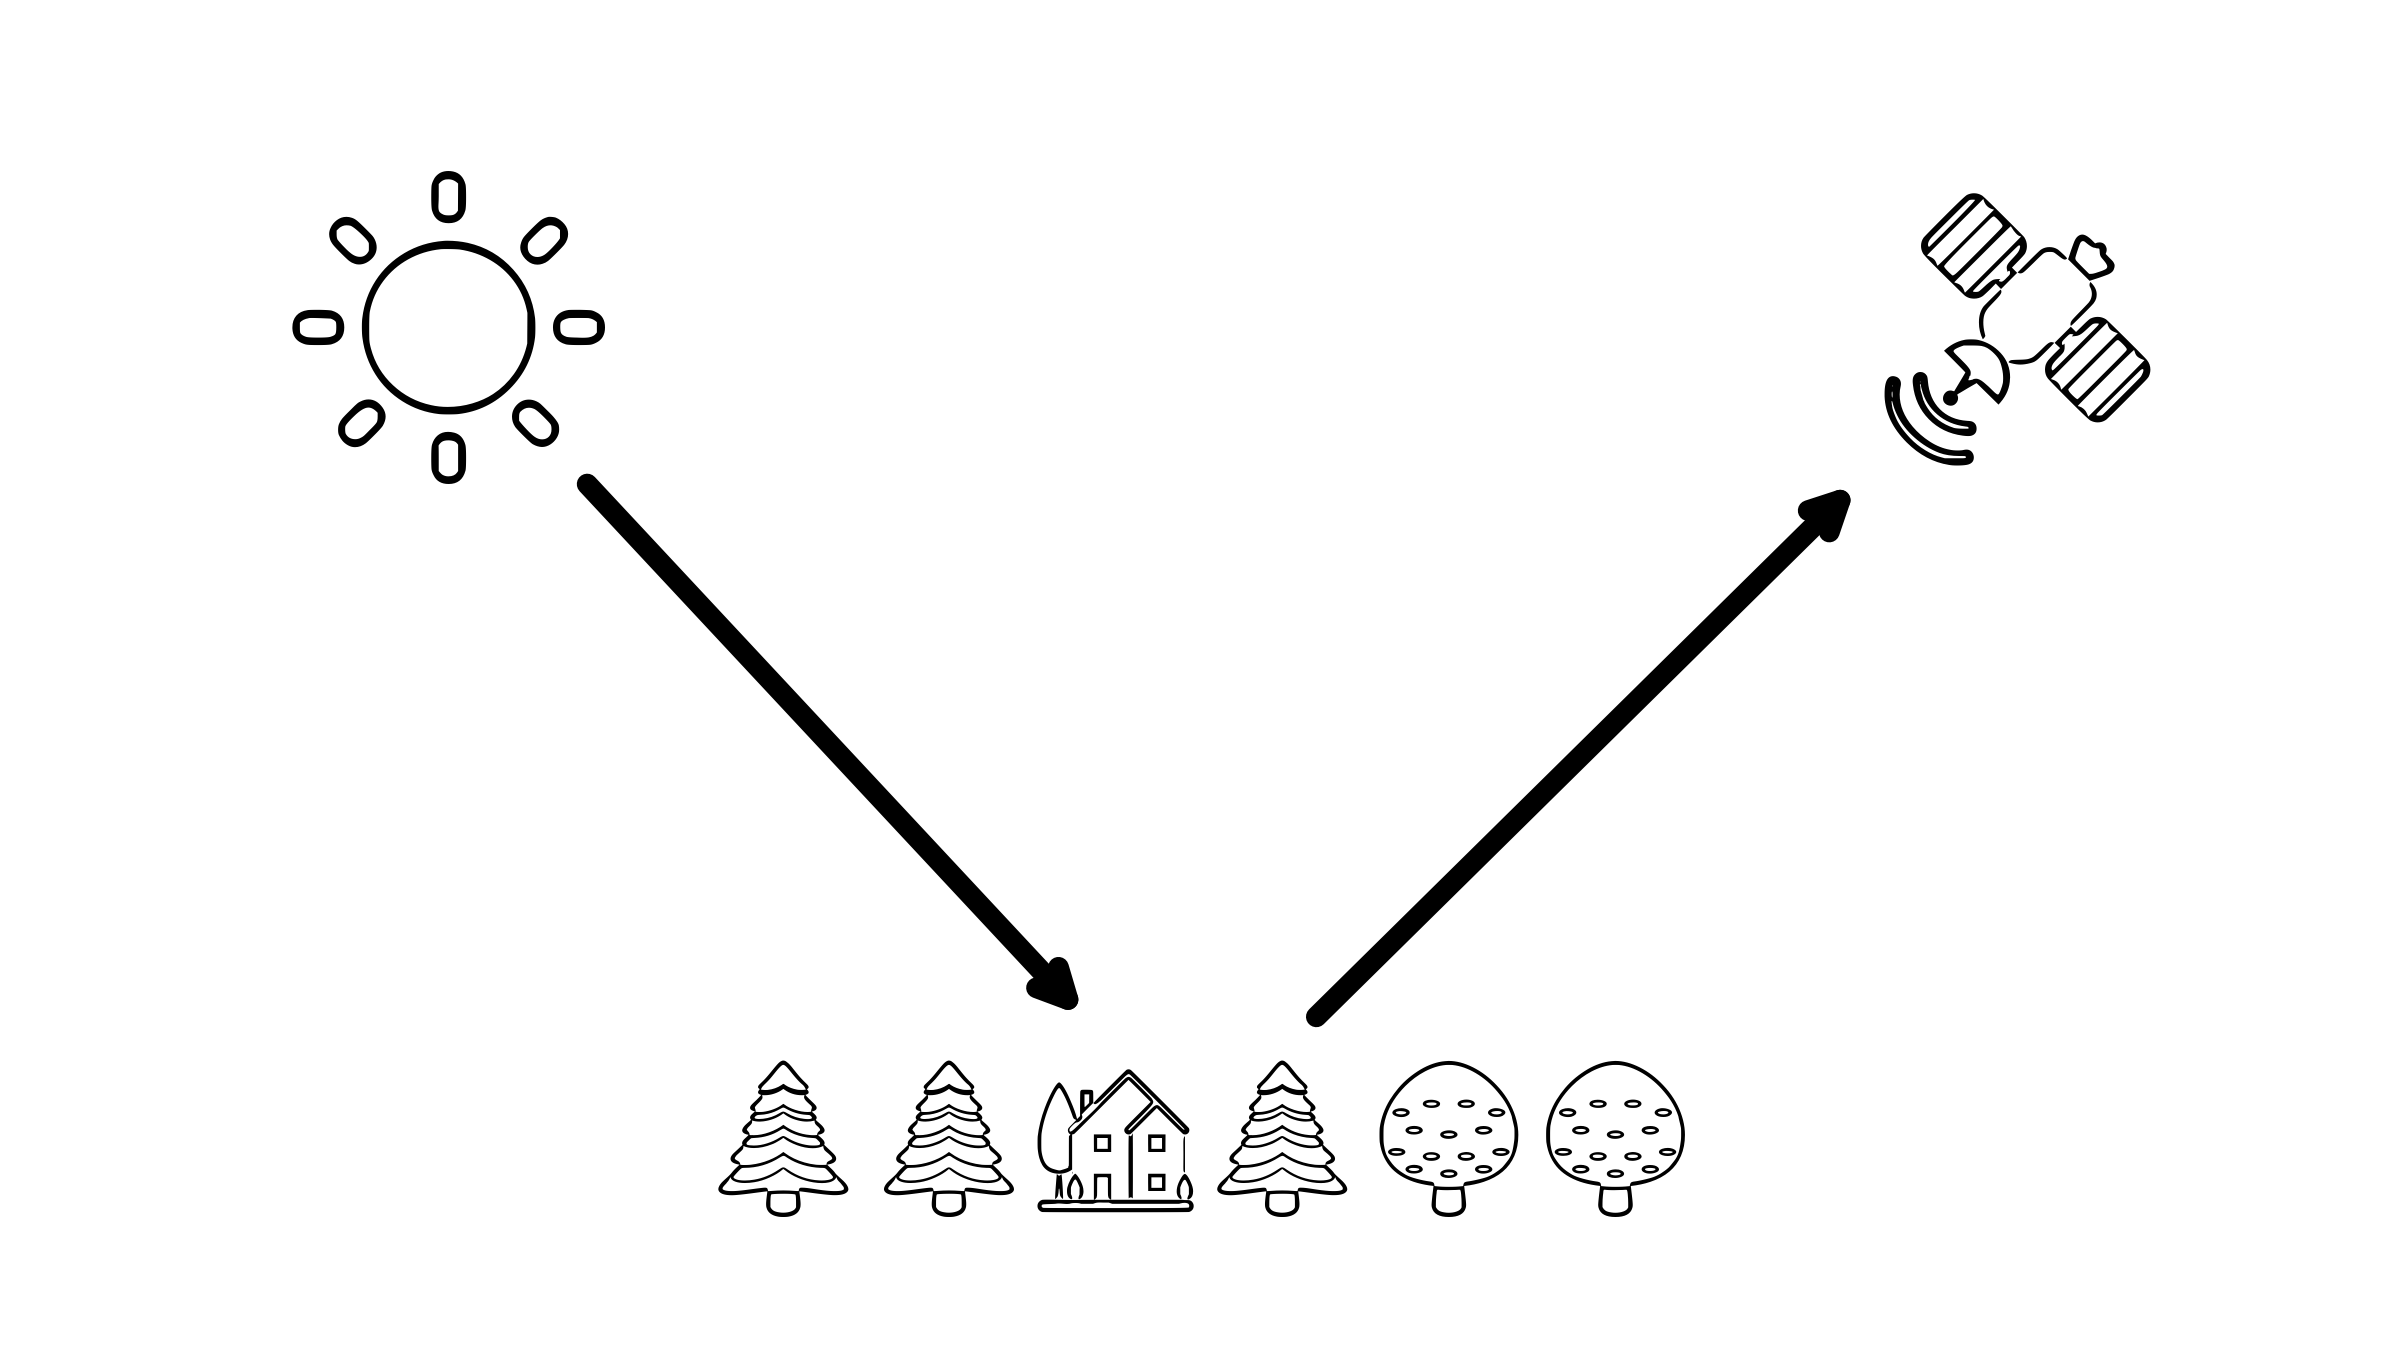
\includegraphics[width=0.8\textwidth]{fig:pasivo.png}}{./figs/fig:pasivo.mp4}
    \caption{Adquisición de imágenes satelitales: sensores pasivos}
    \label{}
  \end{figure}
\end{frame}
%--- Next Frame ---%

\begin{frame}{}
  \begin{figure}
    \centering
    \movie[width = 0.8\textwidth,loop,autostart]{\centering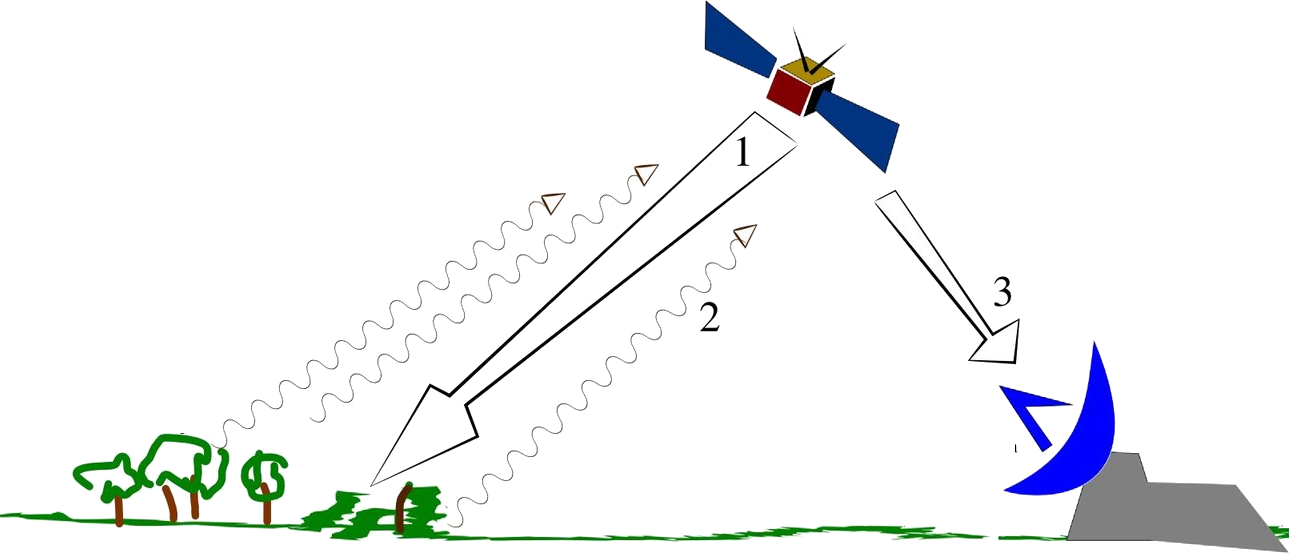
\includegraphics[width=0.8\textwidth]{fig:activo.png}}{./figs/fig:activo.mp4}
    \caption{Adquisición de imágenes satelitales: sensores activos}
    \label{}
  \end{figure}
\end{frame}
%--- Next Frame ---%

\begin{frame}{}
  Algunos ejemplos de plataformas y sensores pasivos:
  \begin{itemize}
    \item<1->{Landsat 5 - TM}
    \item<2-> Landsat 7 - ETM
    \item<3-> Landsat 8 - OLI,TIRS
    \item<4-> TERRA - MODIS, ASTER, CERES, MISR, MOPITT
    \item<5-> AQUA - MODIS, AIRS, AMSU, CERES, AMSR-E, HSB
    \item<6-> Sentinel 2A - MSI
    \item<7-> Sentinel 2B - MSI
    \item<8-> Sentinel 3A - SLSRT, OLCI, SRAL, DORIS, MWR, LRR, GNSS
  \end{itemize}
\end{frame}
%--- Next Frame ---%

\begin{frame}{}
\only<1>{Tipos de órbitas.}
\only<2->{
\begin{block}{Clasificación de órbitas}
   Una órbita es el camino que recorre un cuerpo en el espacio. Las dos más importantes en teledetección son:
   \begin{itemize}
     \item \emph{Polares}: Orbitando en torno a la tierra en dirección norte-sur o sur-norte.
     \item \emph{Geoestacionarias}: Orbitando en el mismo sentido y velocidad angular que la tierra.
   \end{itemize}
\end{block}}
\end{frame}
%--- Next Frame ---%

\begin{frame}{}
  \begin{figure}
    \centering
    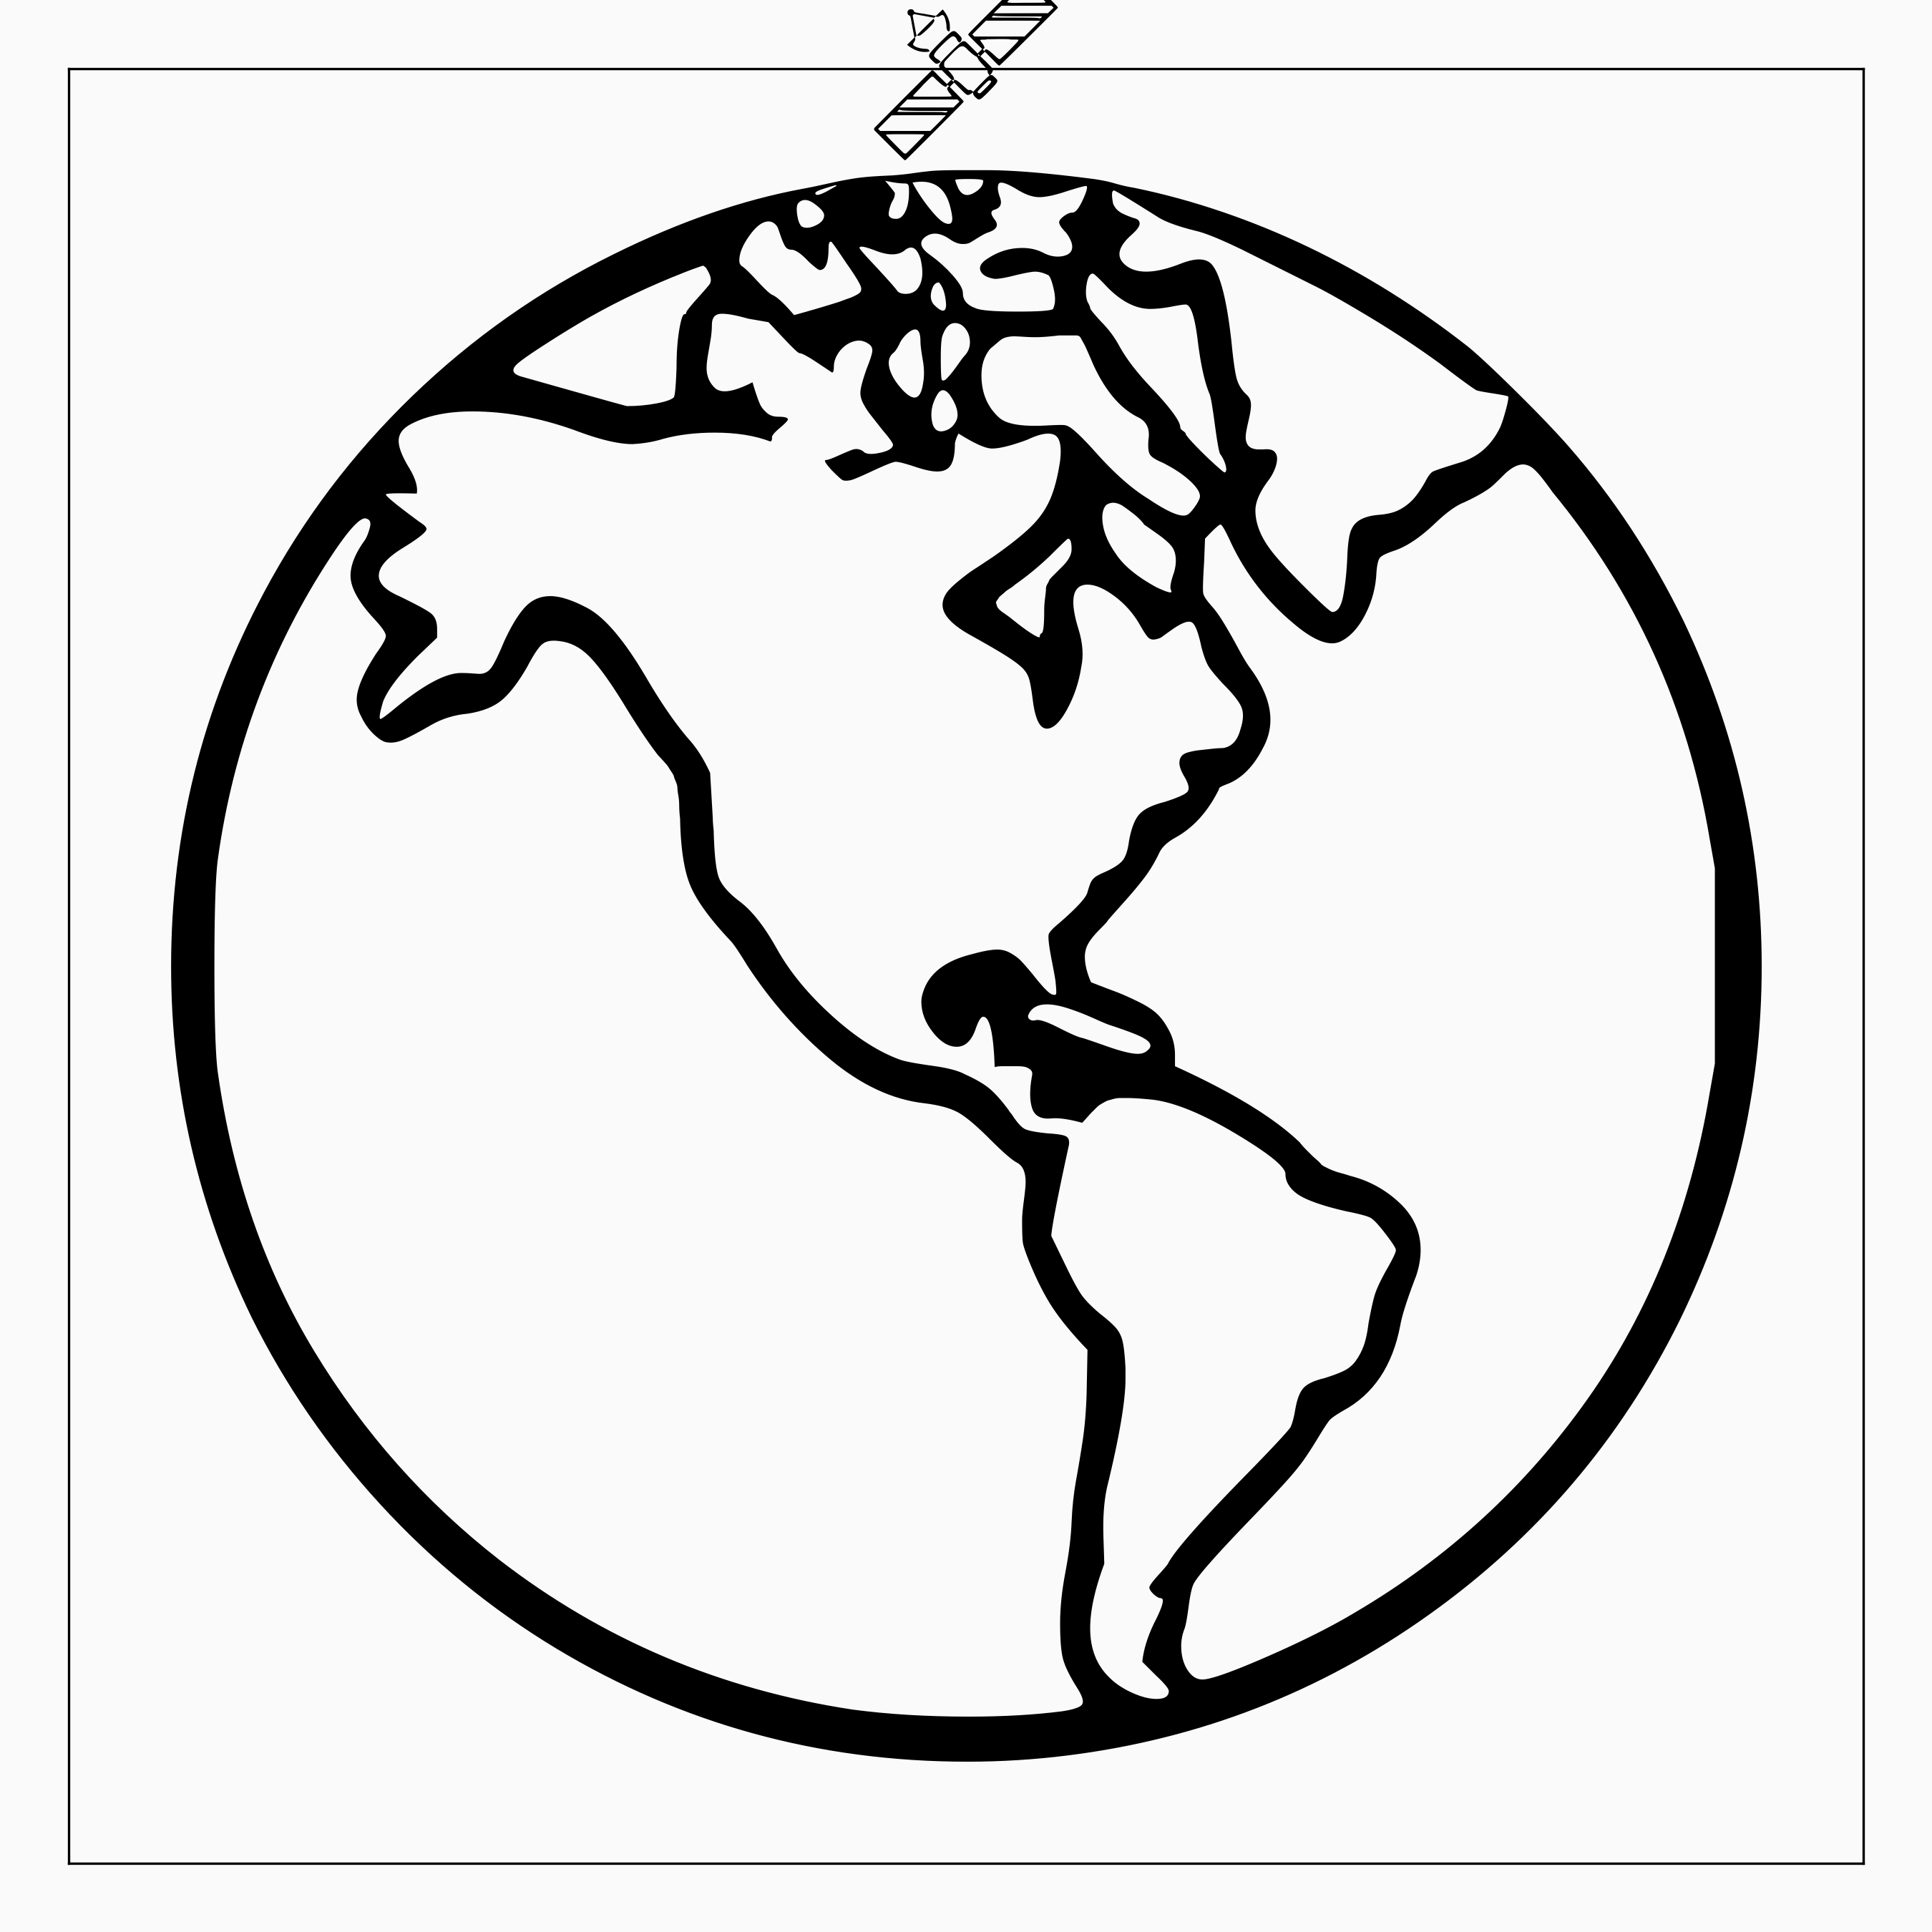
\includegraphics[width=0.8\textwidth]{fig:polar.png}
    \caption{Orbitas polares.}
    \label{}
  \end{figure}
\end{frame}

\begin{frame}{}
  \begin{figure}
    \centering
    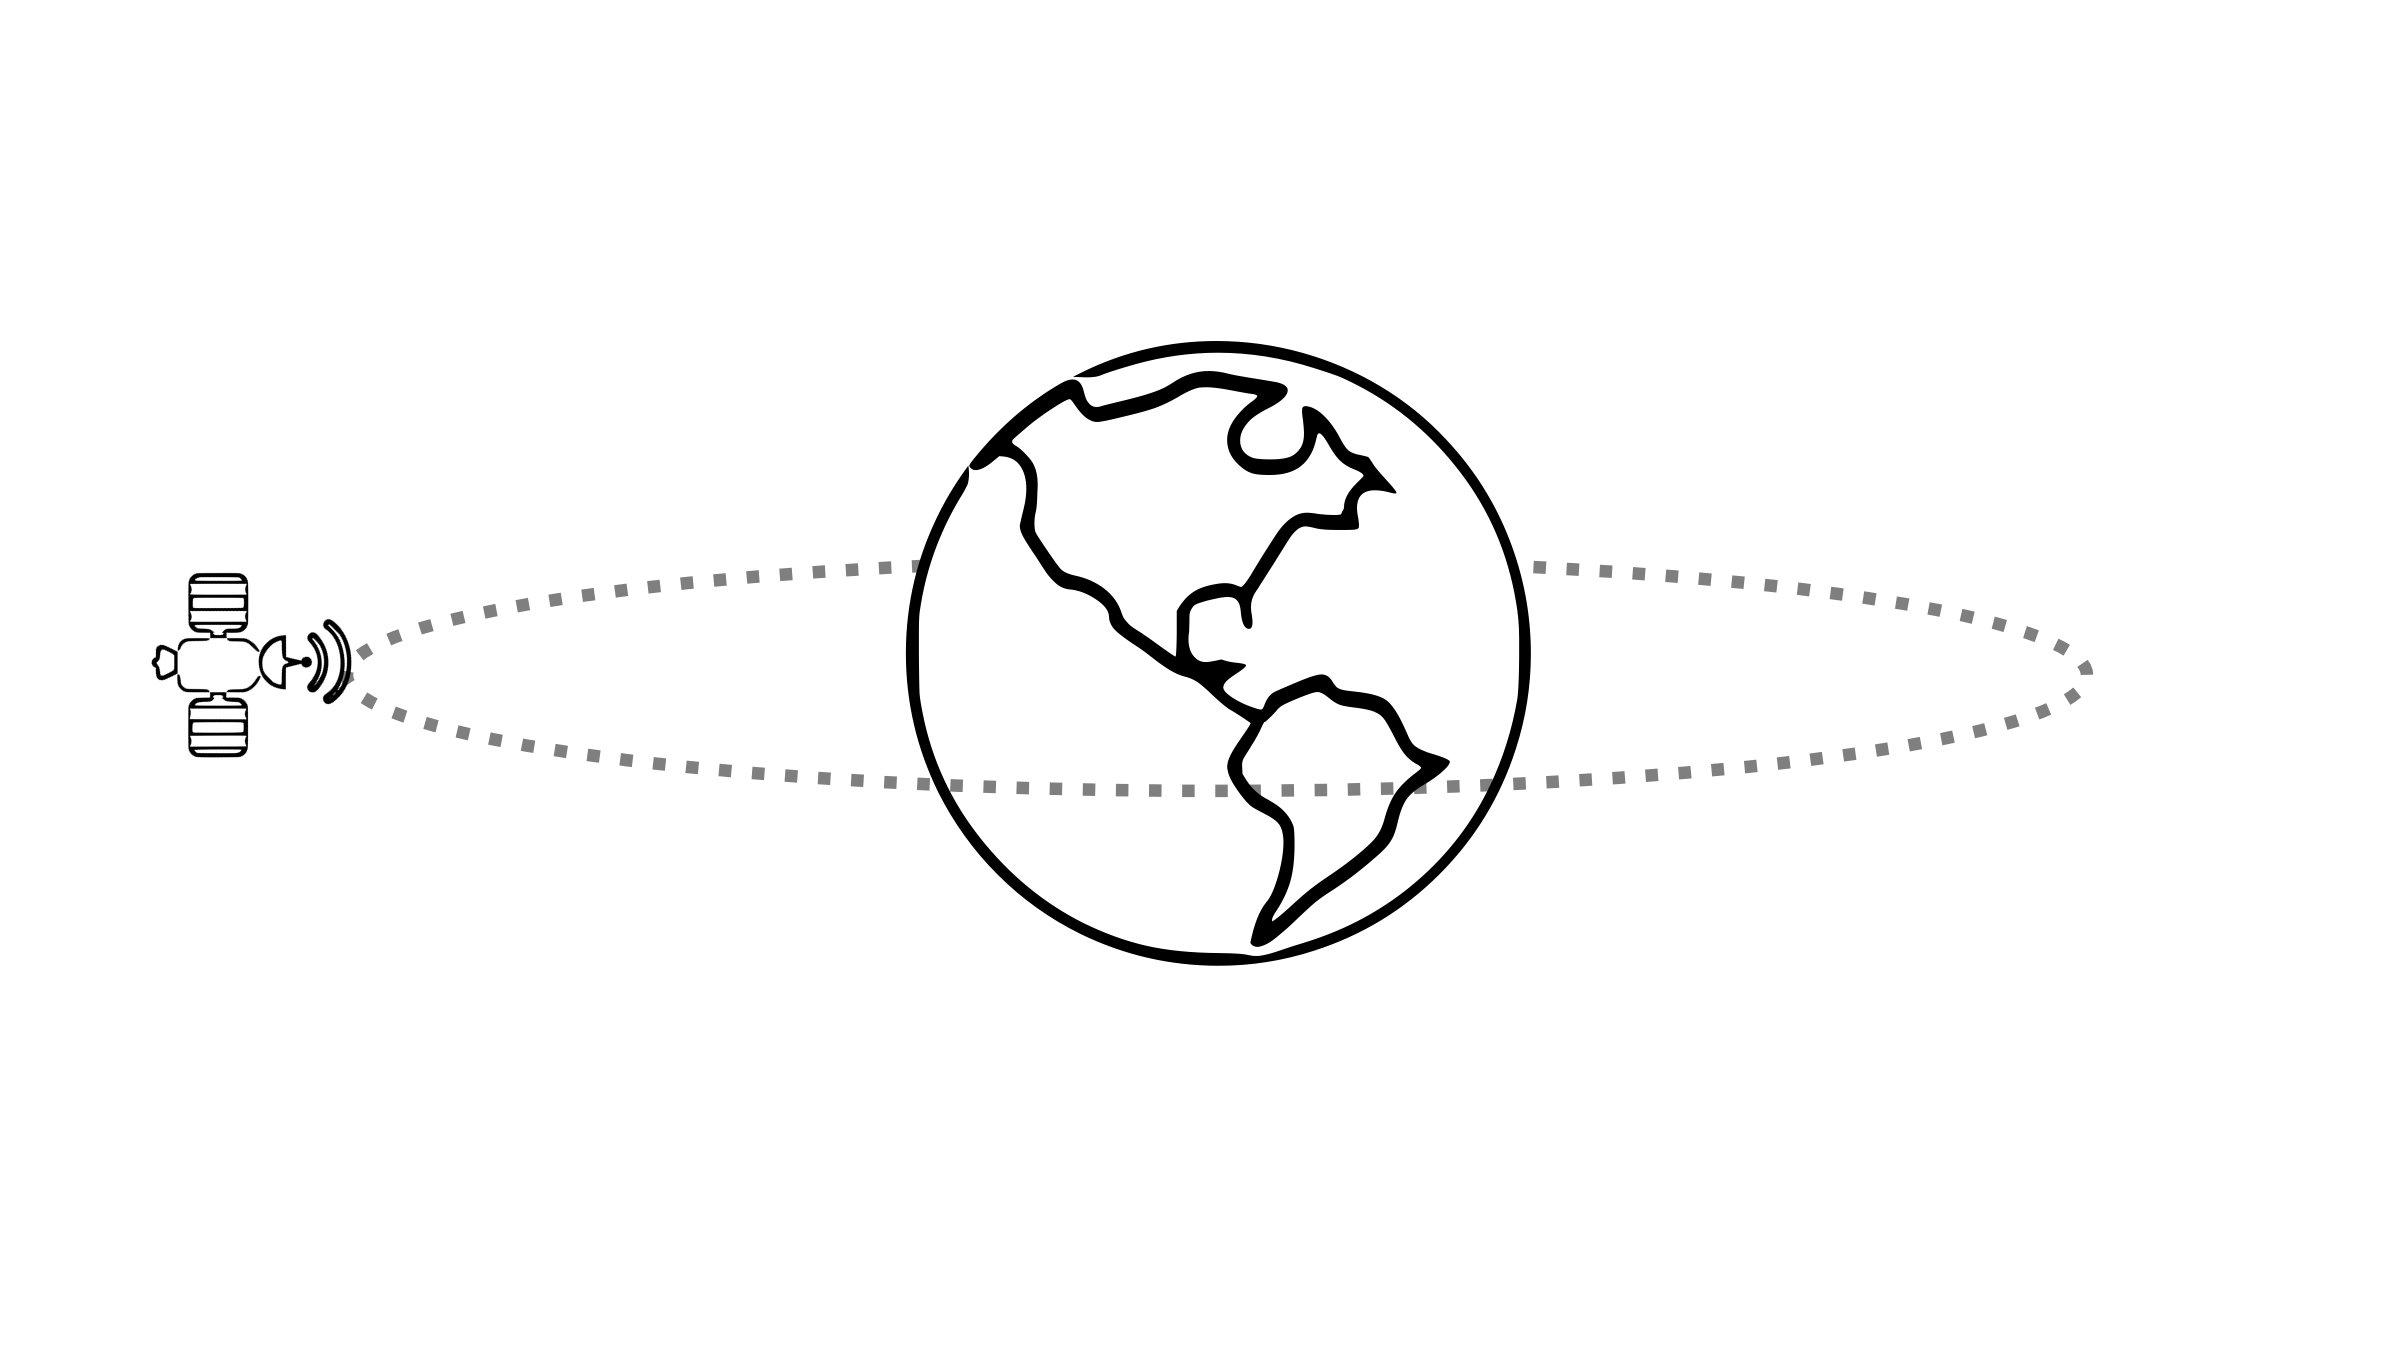
\includegraphics[width=0.8\textwidth]{fig:geo.png}
    \caption{Orbitas geoestacionarias.}
    \label{}
  \end{figure}
\end{frame}
%--- Next Frame ---%
\begin{frame}{}
\only<1>{Resolución espacial.}

\end{frame}

%--- Next Frame ---%

\begin{frame}{}
    \begin{block}{Definición}
        Es la capacidad del sensor de distinguir objetos en el terreno.%ver definición
    \end{block}
                                                                                                                                                                                                                                                                                                                                                                                                                                                                                                                                                                                                                                                                                                                                                                                                                                                                                                                                                                                                                                                                                                                                                                                                                                                                                                                                                                                                                                                                                                                                                                                                                                                                                                                                                                                                                                                                                                                                                                                                                                                                                                                                                              \end{frame}

\subsection{Resolución espacial y temporal}

\begin{frame}{}
  \begin{figure}
    \centering
    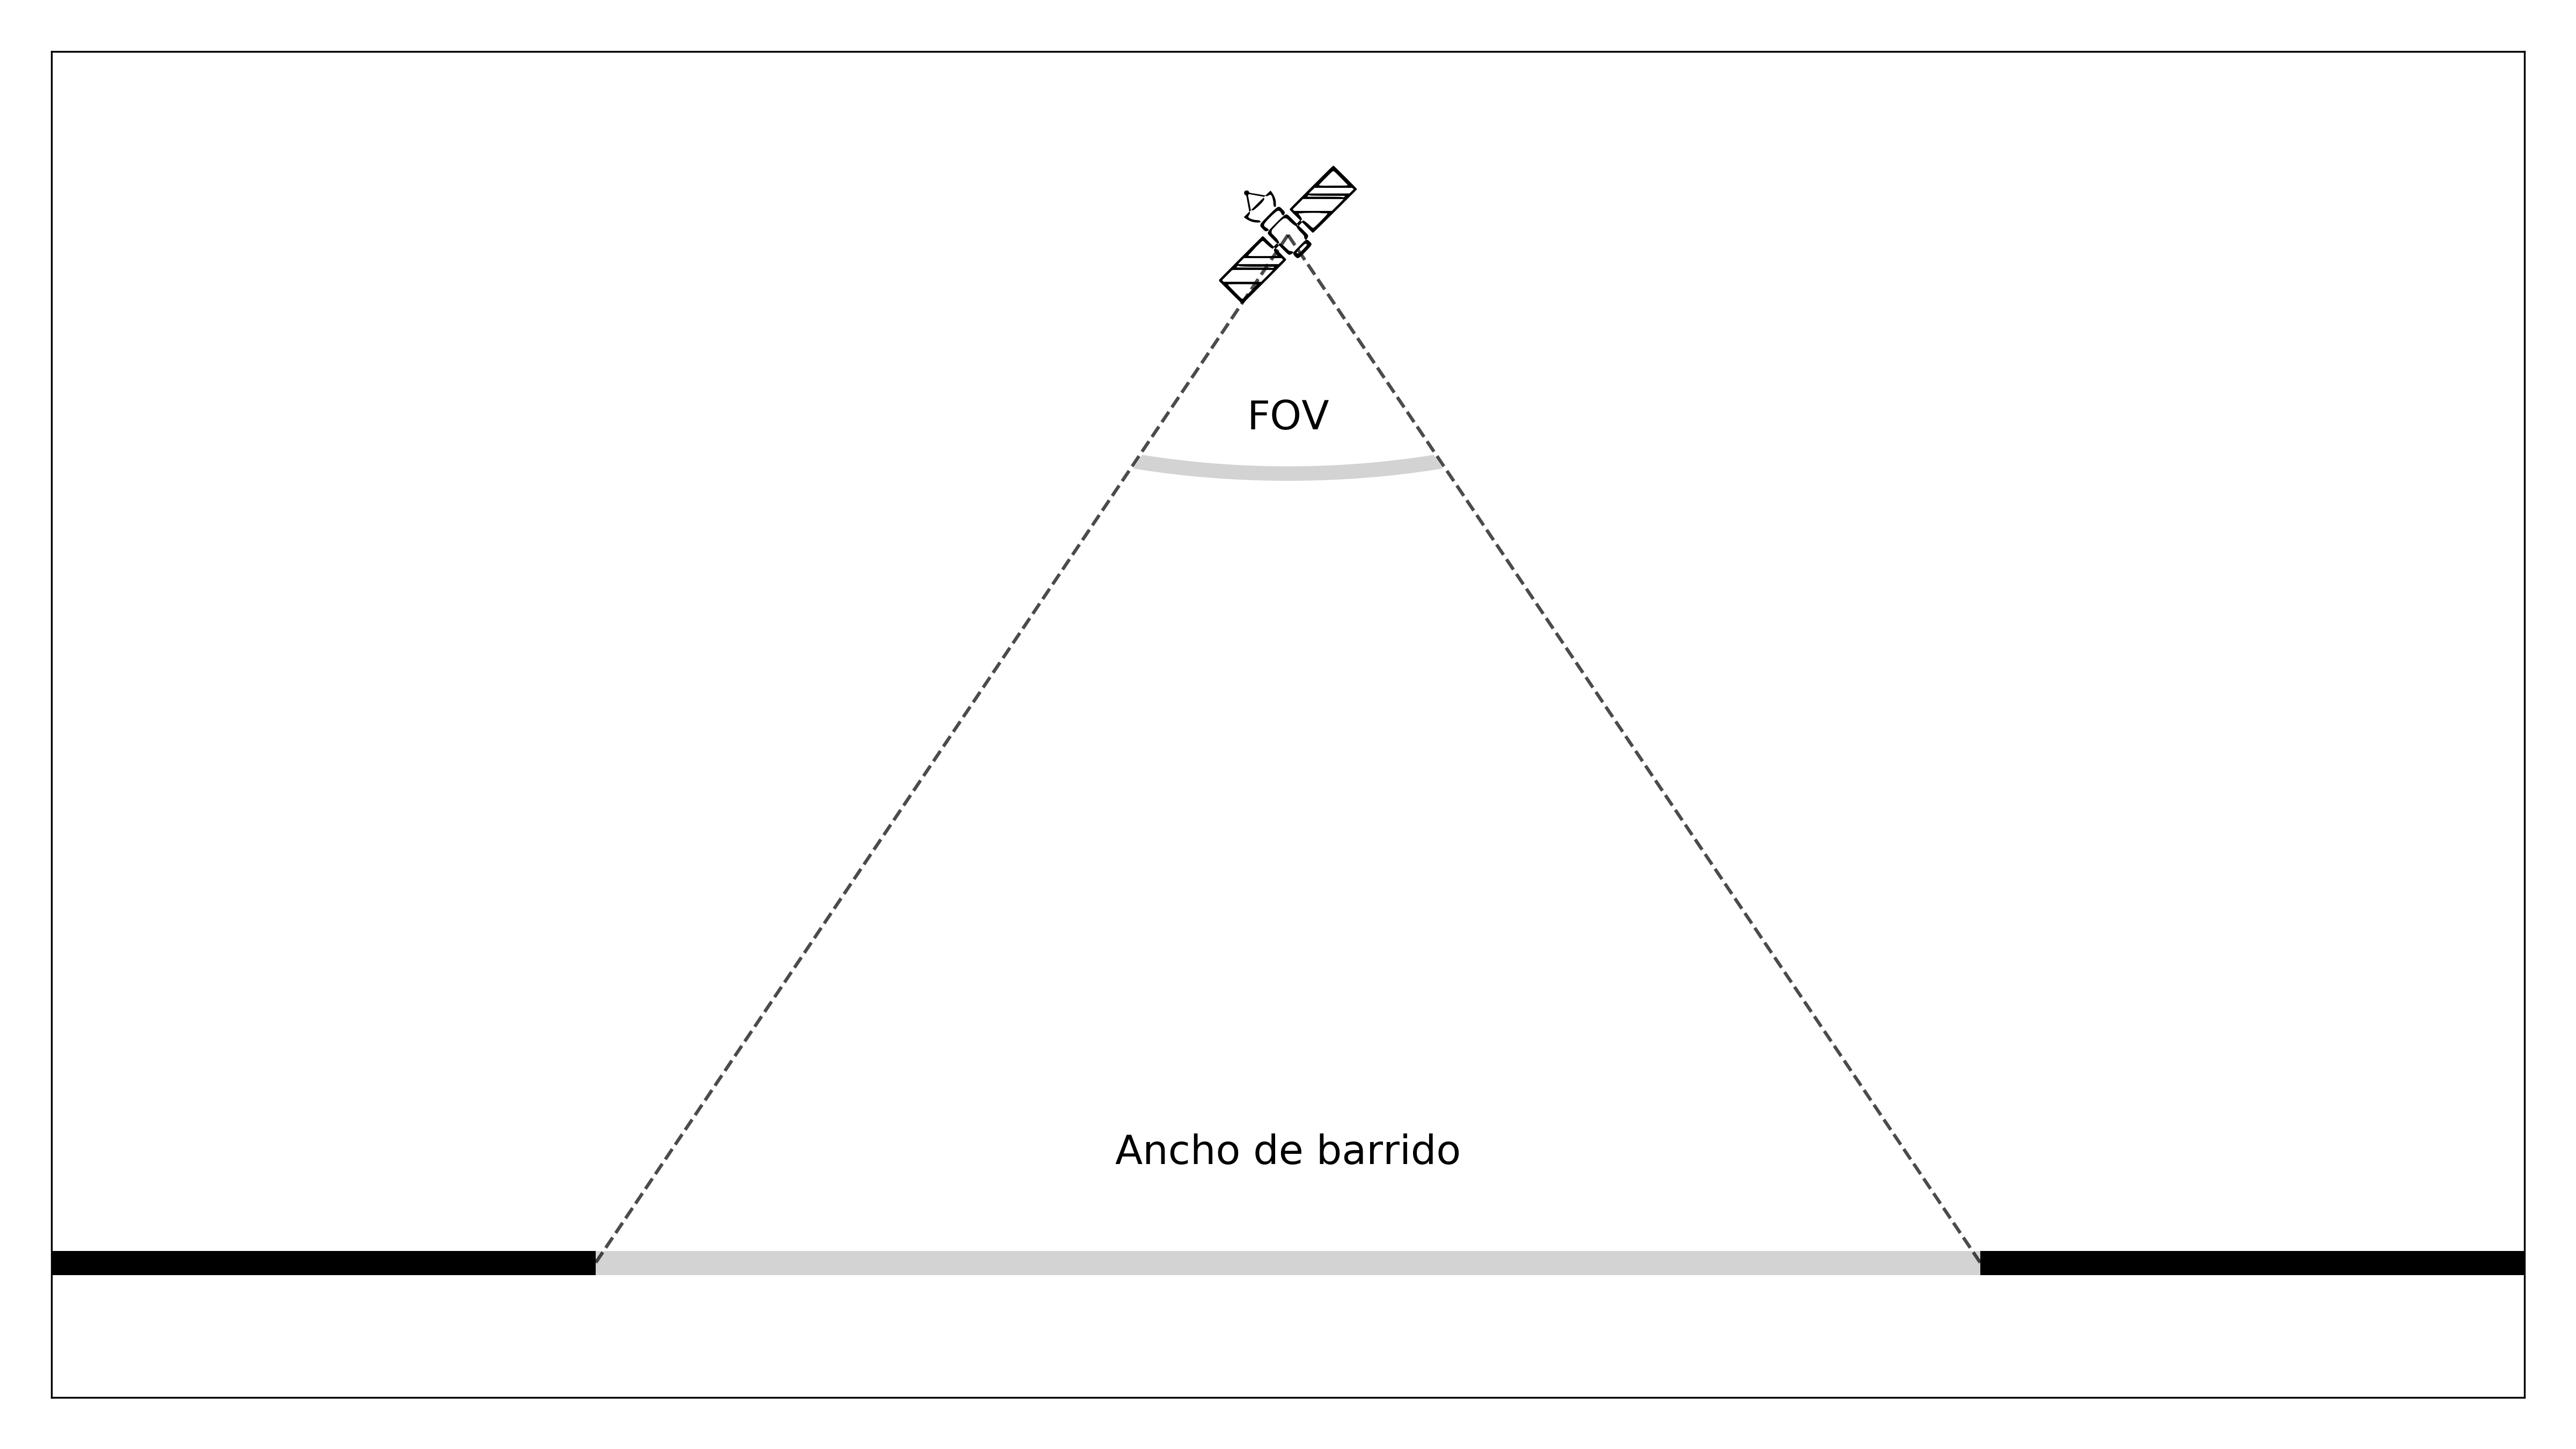
\includegraphics[width=0.8\textwidth]{fig:anchobarrido.png}
    \caption{Ancho de barrido.}
    \label{}
  \end{figure}
\end{frame}
%--- Next Frame ---%

\begin{frame}{}
  \begin{figure}
    \centering
    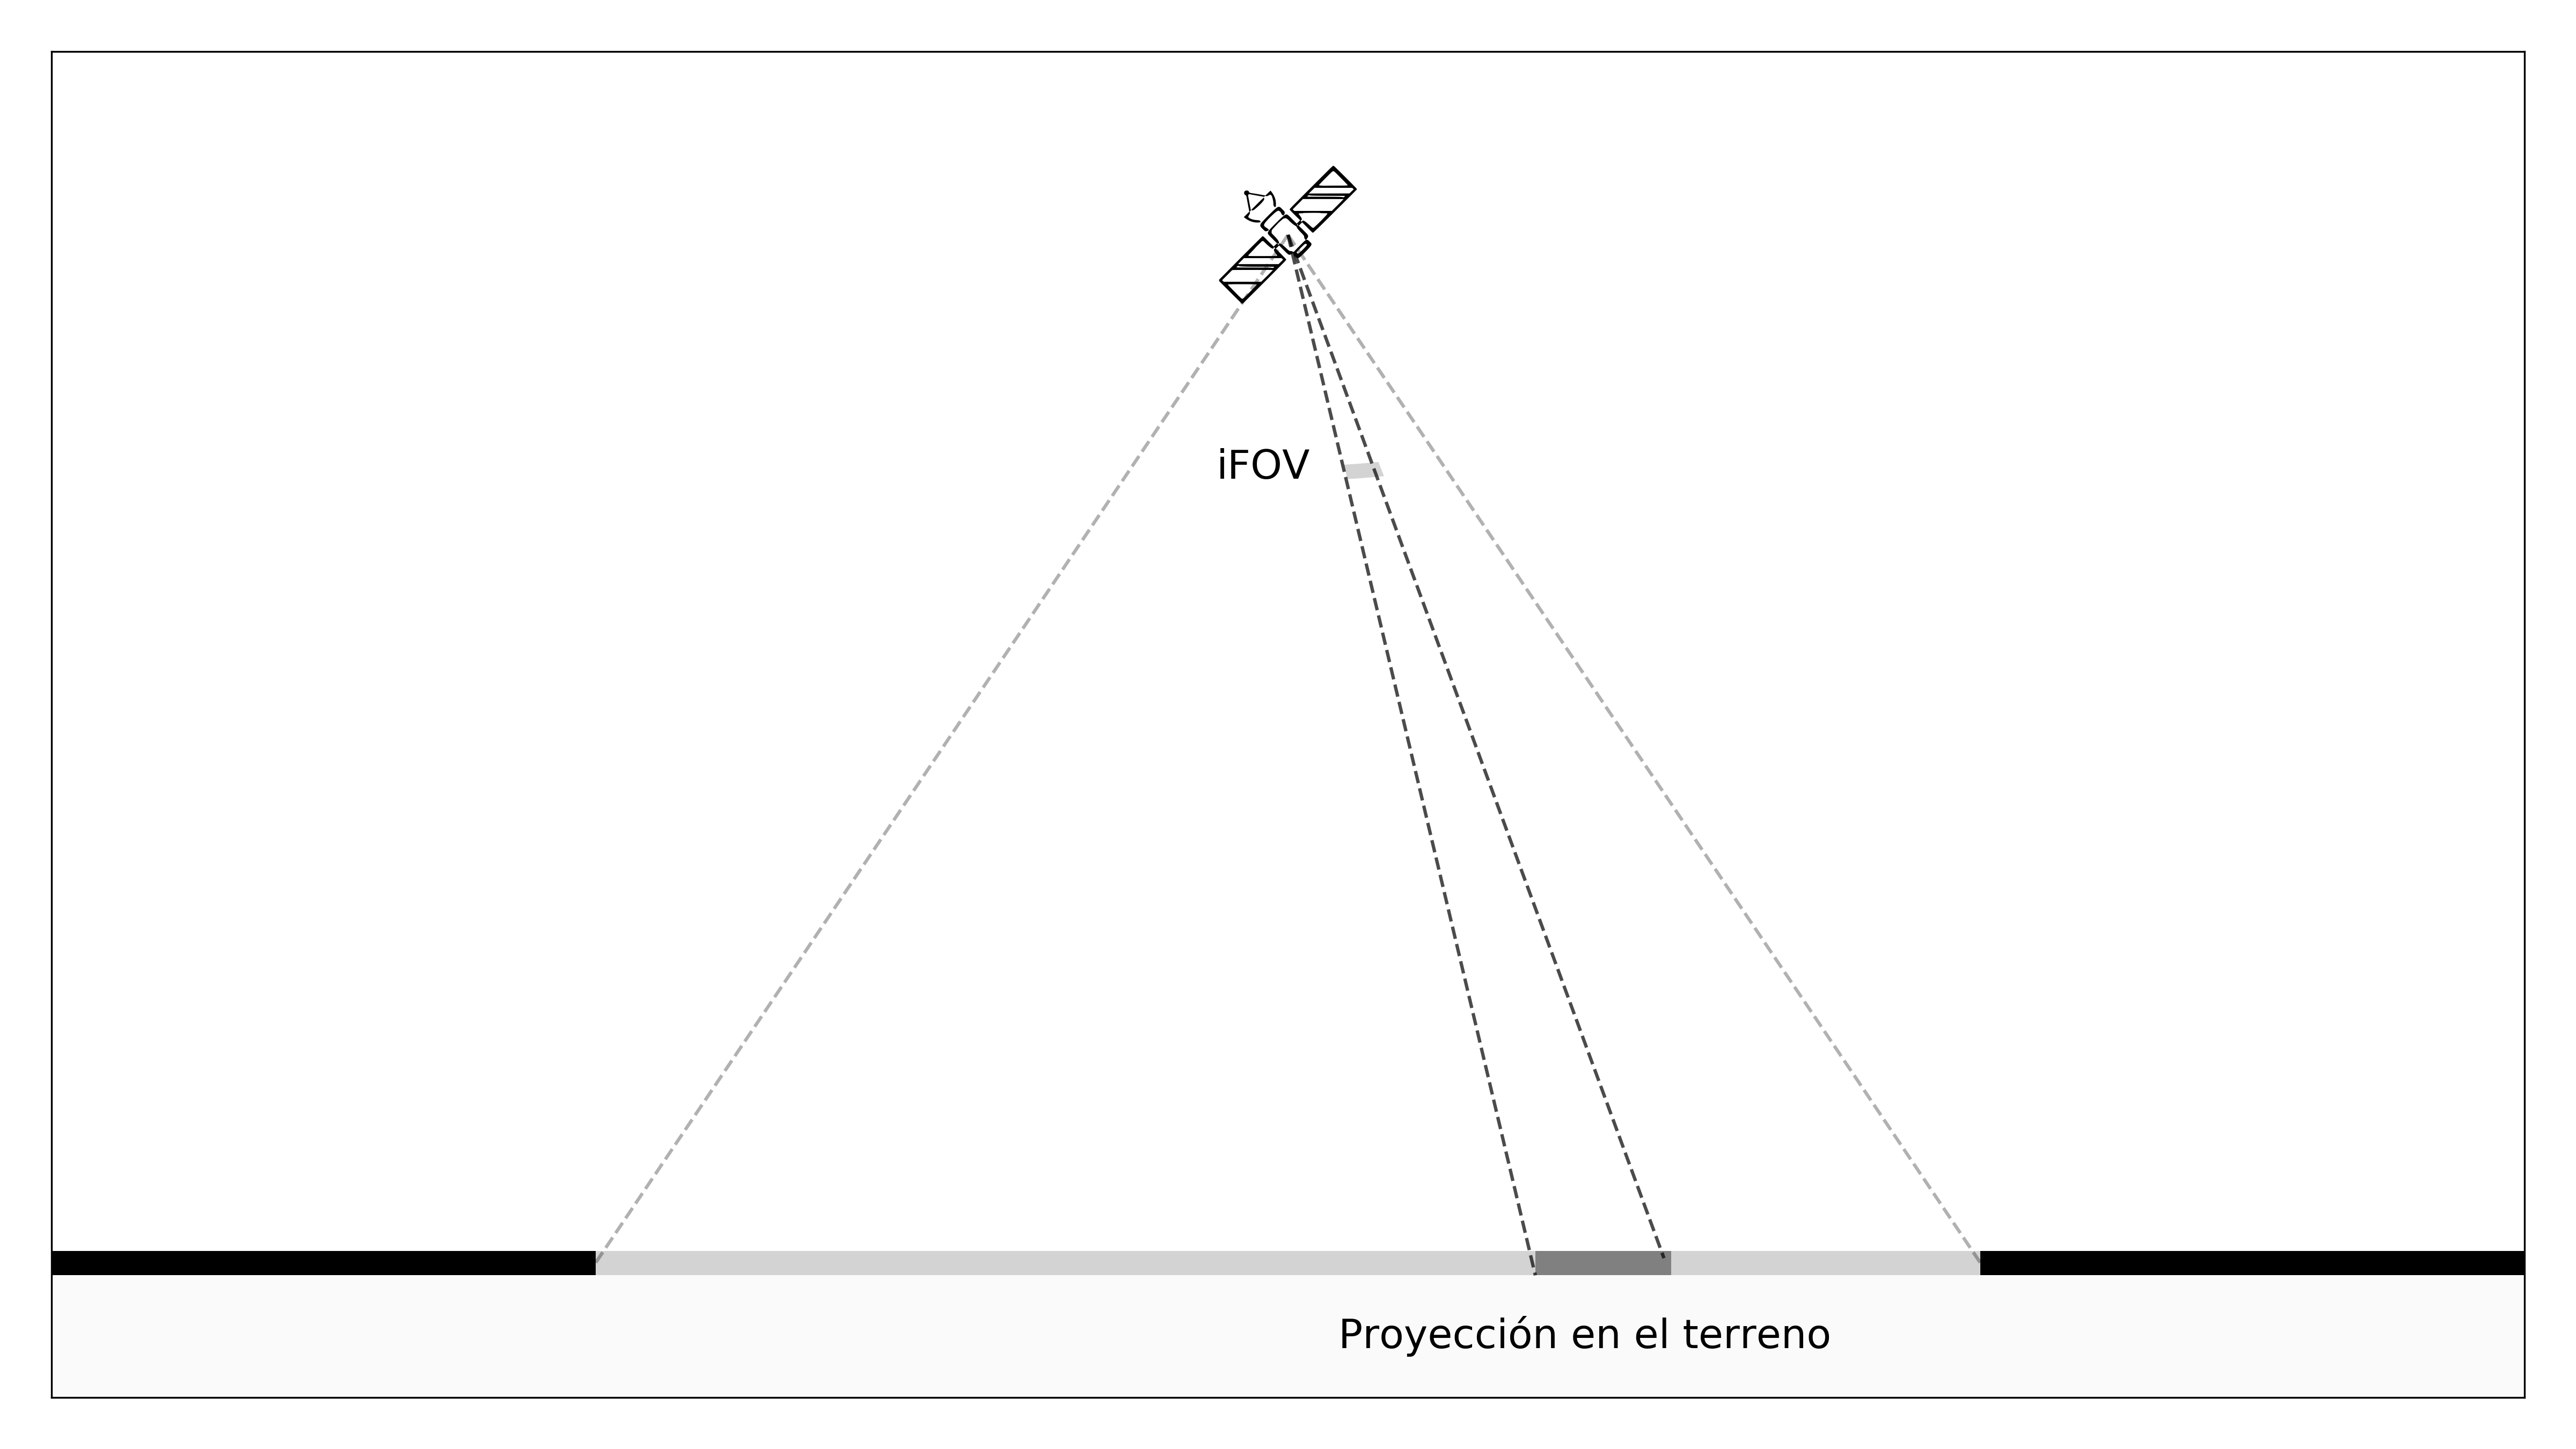
\includegraphics[width=0.7\textwidth]{fig:resolucion1.png}
    \caption{Resolución proyectada en el terreno.}
    \label{}
  \end{figure}
\end{frame}
%--- Next Frame ---%


%\begin{frame}{}
 %   \begin{figure}[h!]
  %      \centering
   %     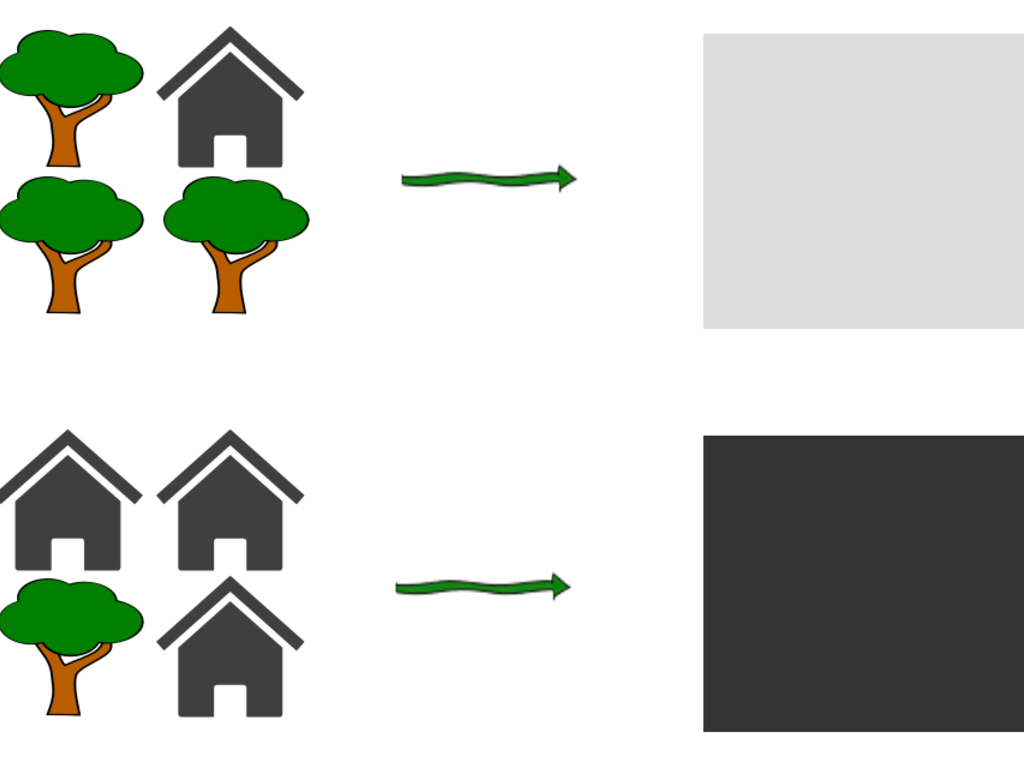
\includegraphics[width=0.5\textwidth]{fig:pixel.png}
    %    \caption{Formación de una celda de informacion.}
%    \end{figure}
%\end{frame}

%--- Next Frame ---%

\begin{frame}{}
  \begin{figure}
    \centering
    \movie[width = 0.8\textwidth,loop,autostart]{\centering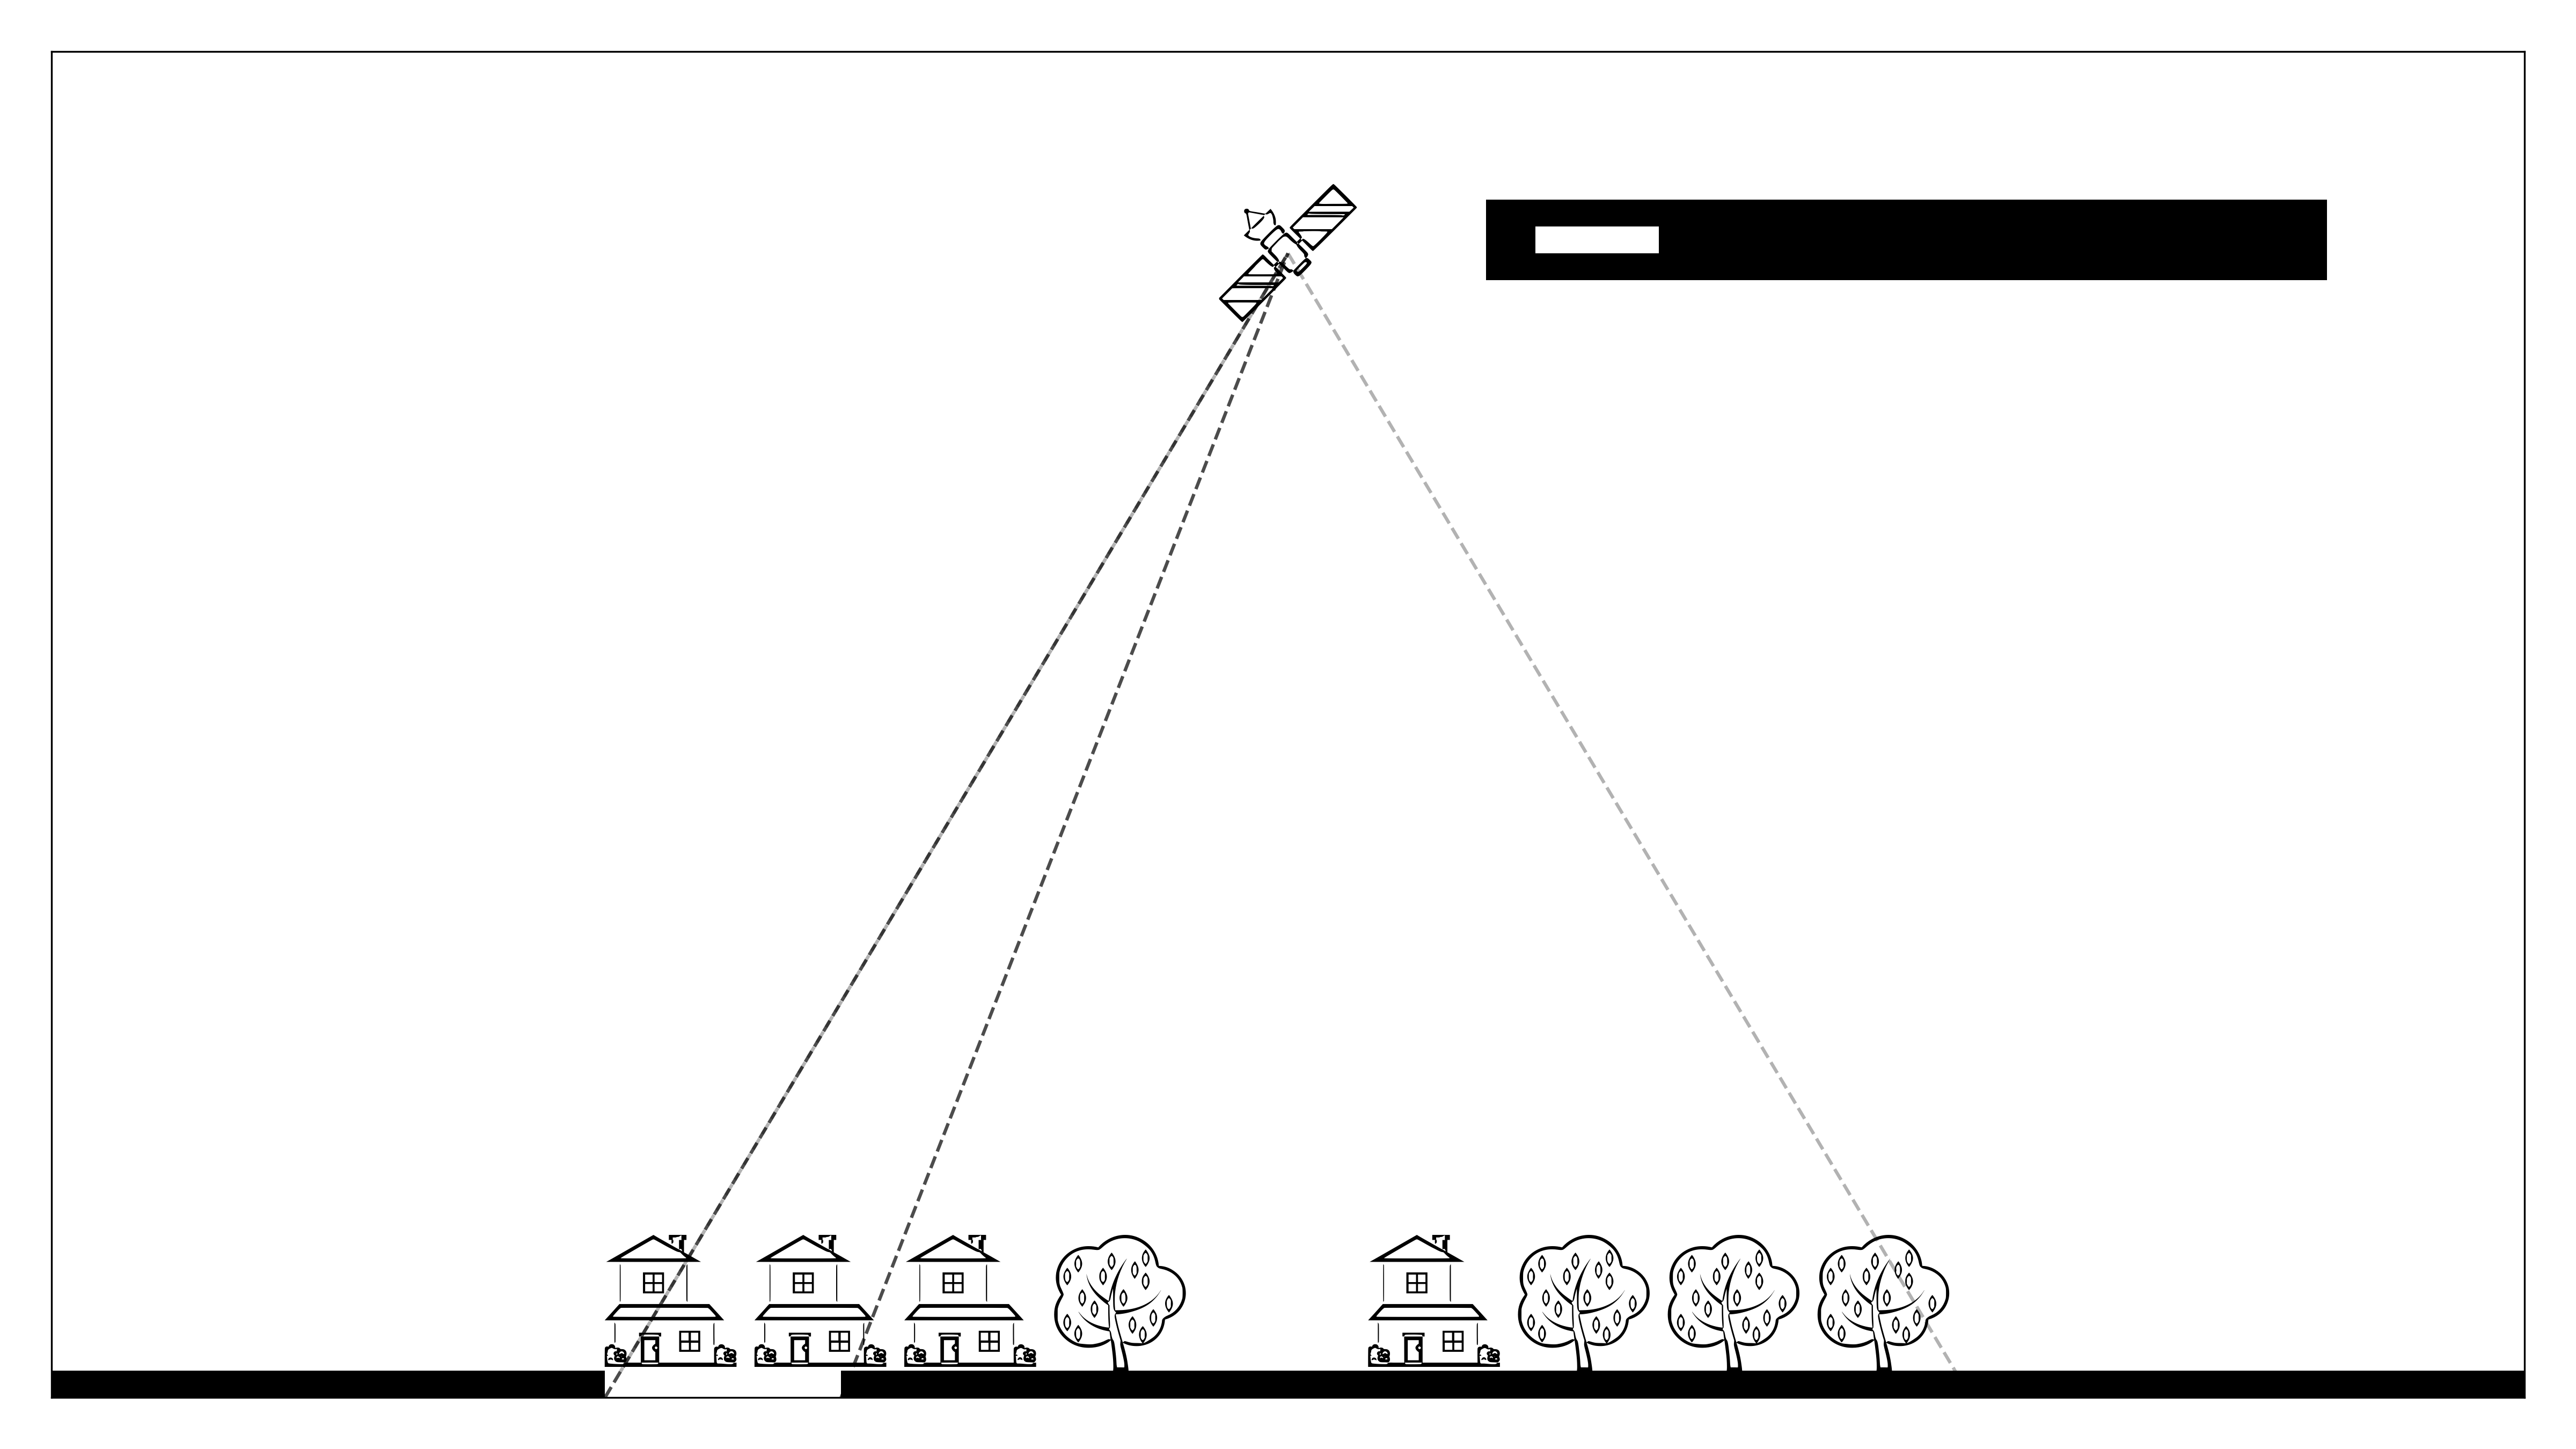
\includegraphics[width=0.8\textwidth]{fig:pixel6.png}}{./figs/fig:pixel6.mp4}
    \caption{Resolución proyectada en el terreno.}
    \label{}
  \end{figure}
\end{frame}
%--- Next Frame ---%

\begin{frame}{}
  \begin{figure}
    \centering
    \movie[width = 0.8\textwidth,loop,autostart]{\centering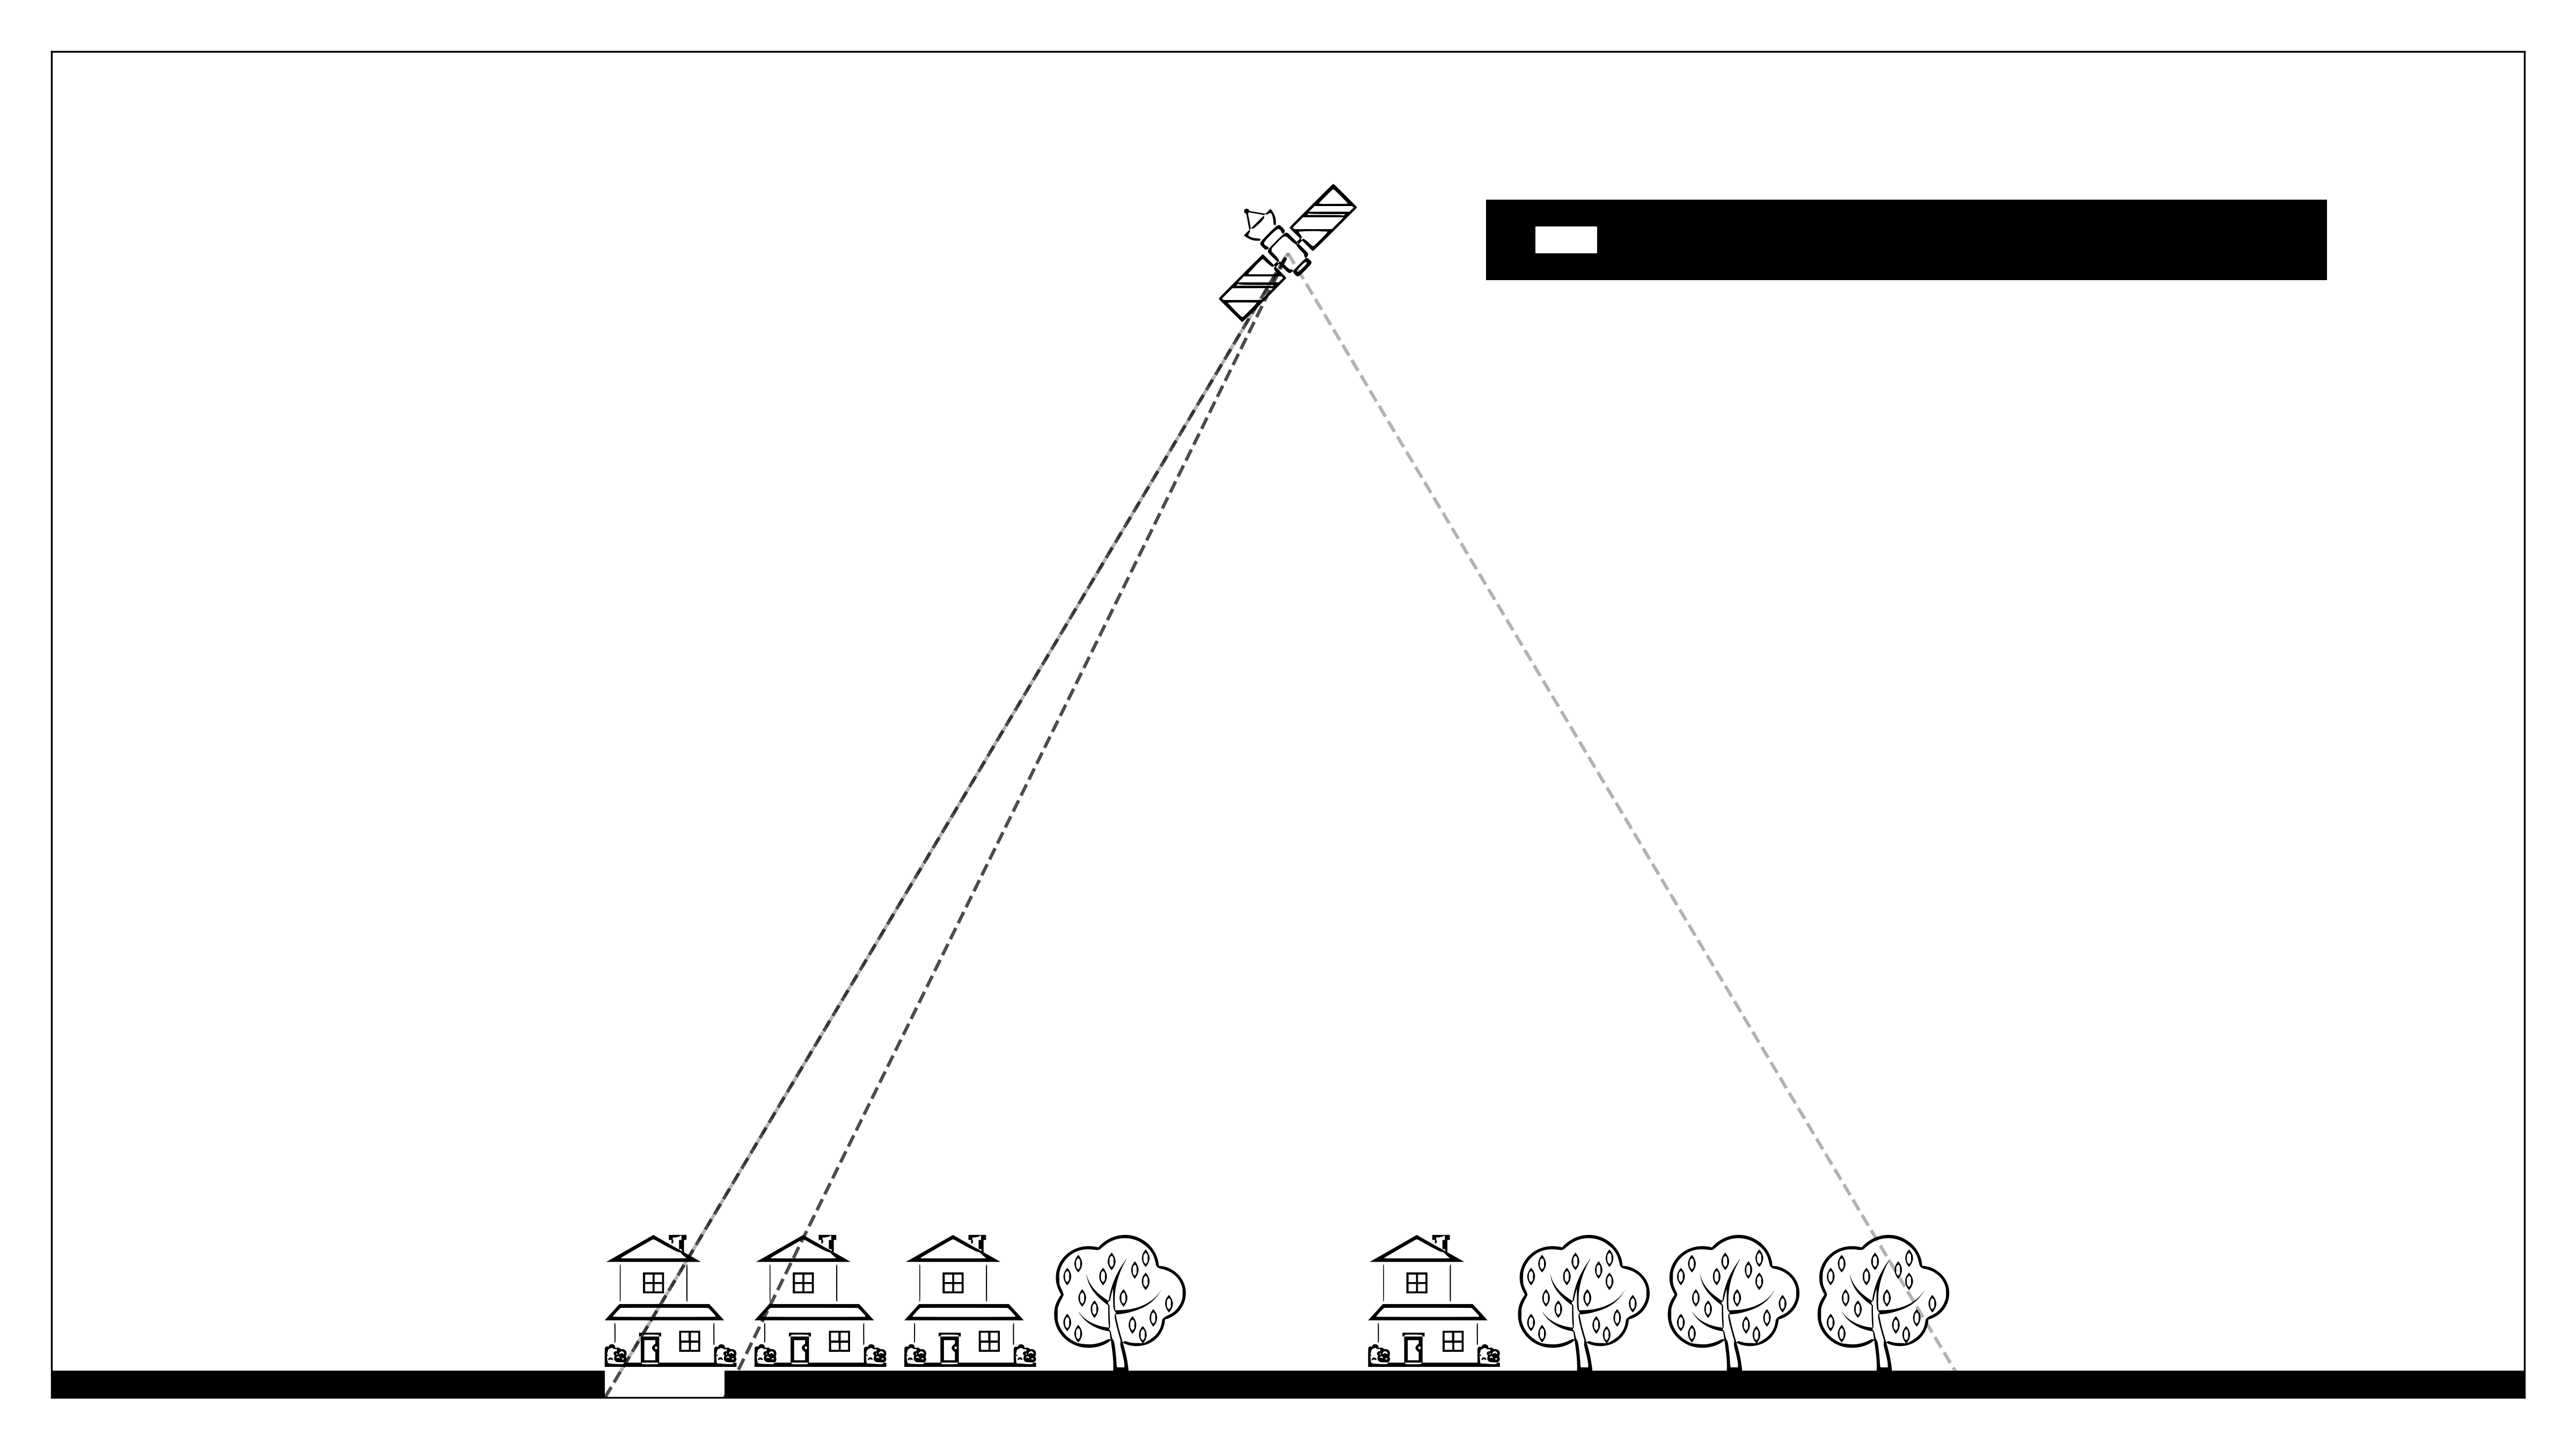
\includegraphics[width=0.8\textwidth]{fig:pixel3.png}}{./figs/fig:pixel3.mp4}
    \caption{Resolución proyectada en el terreno.}
    \label{}
  \end{figure}
\end{frame}
%--- Next Frame ---%

\begin{frame}{}
  \begin{figure}
    \centering
    \movie[width = 0.8\textwidth,loop,autostart]{\centering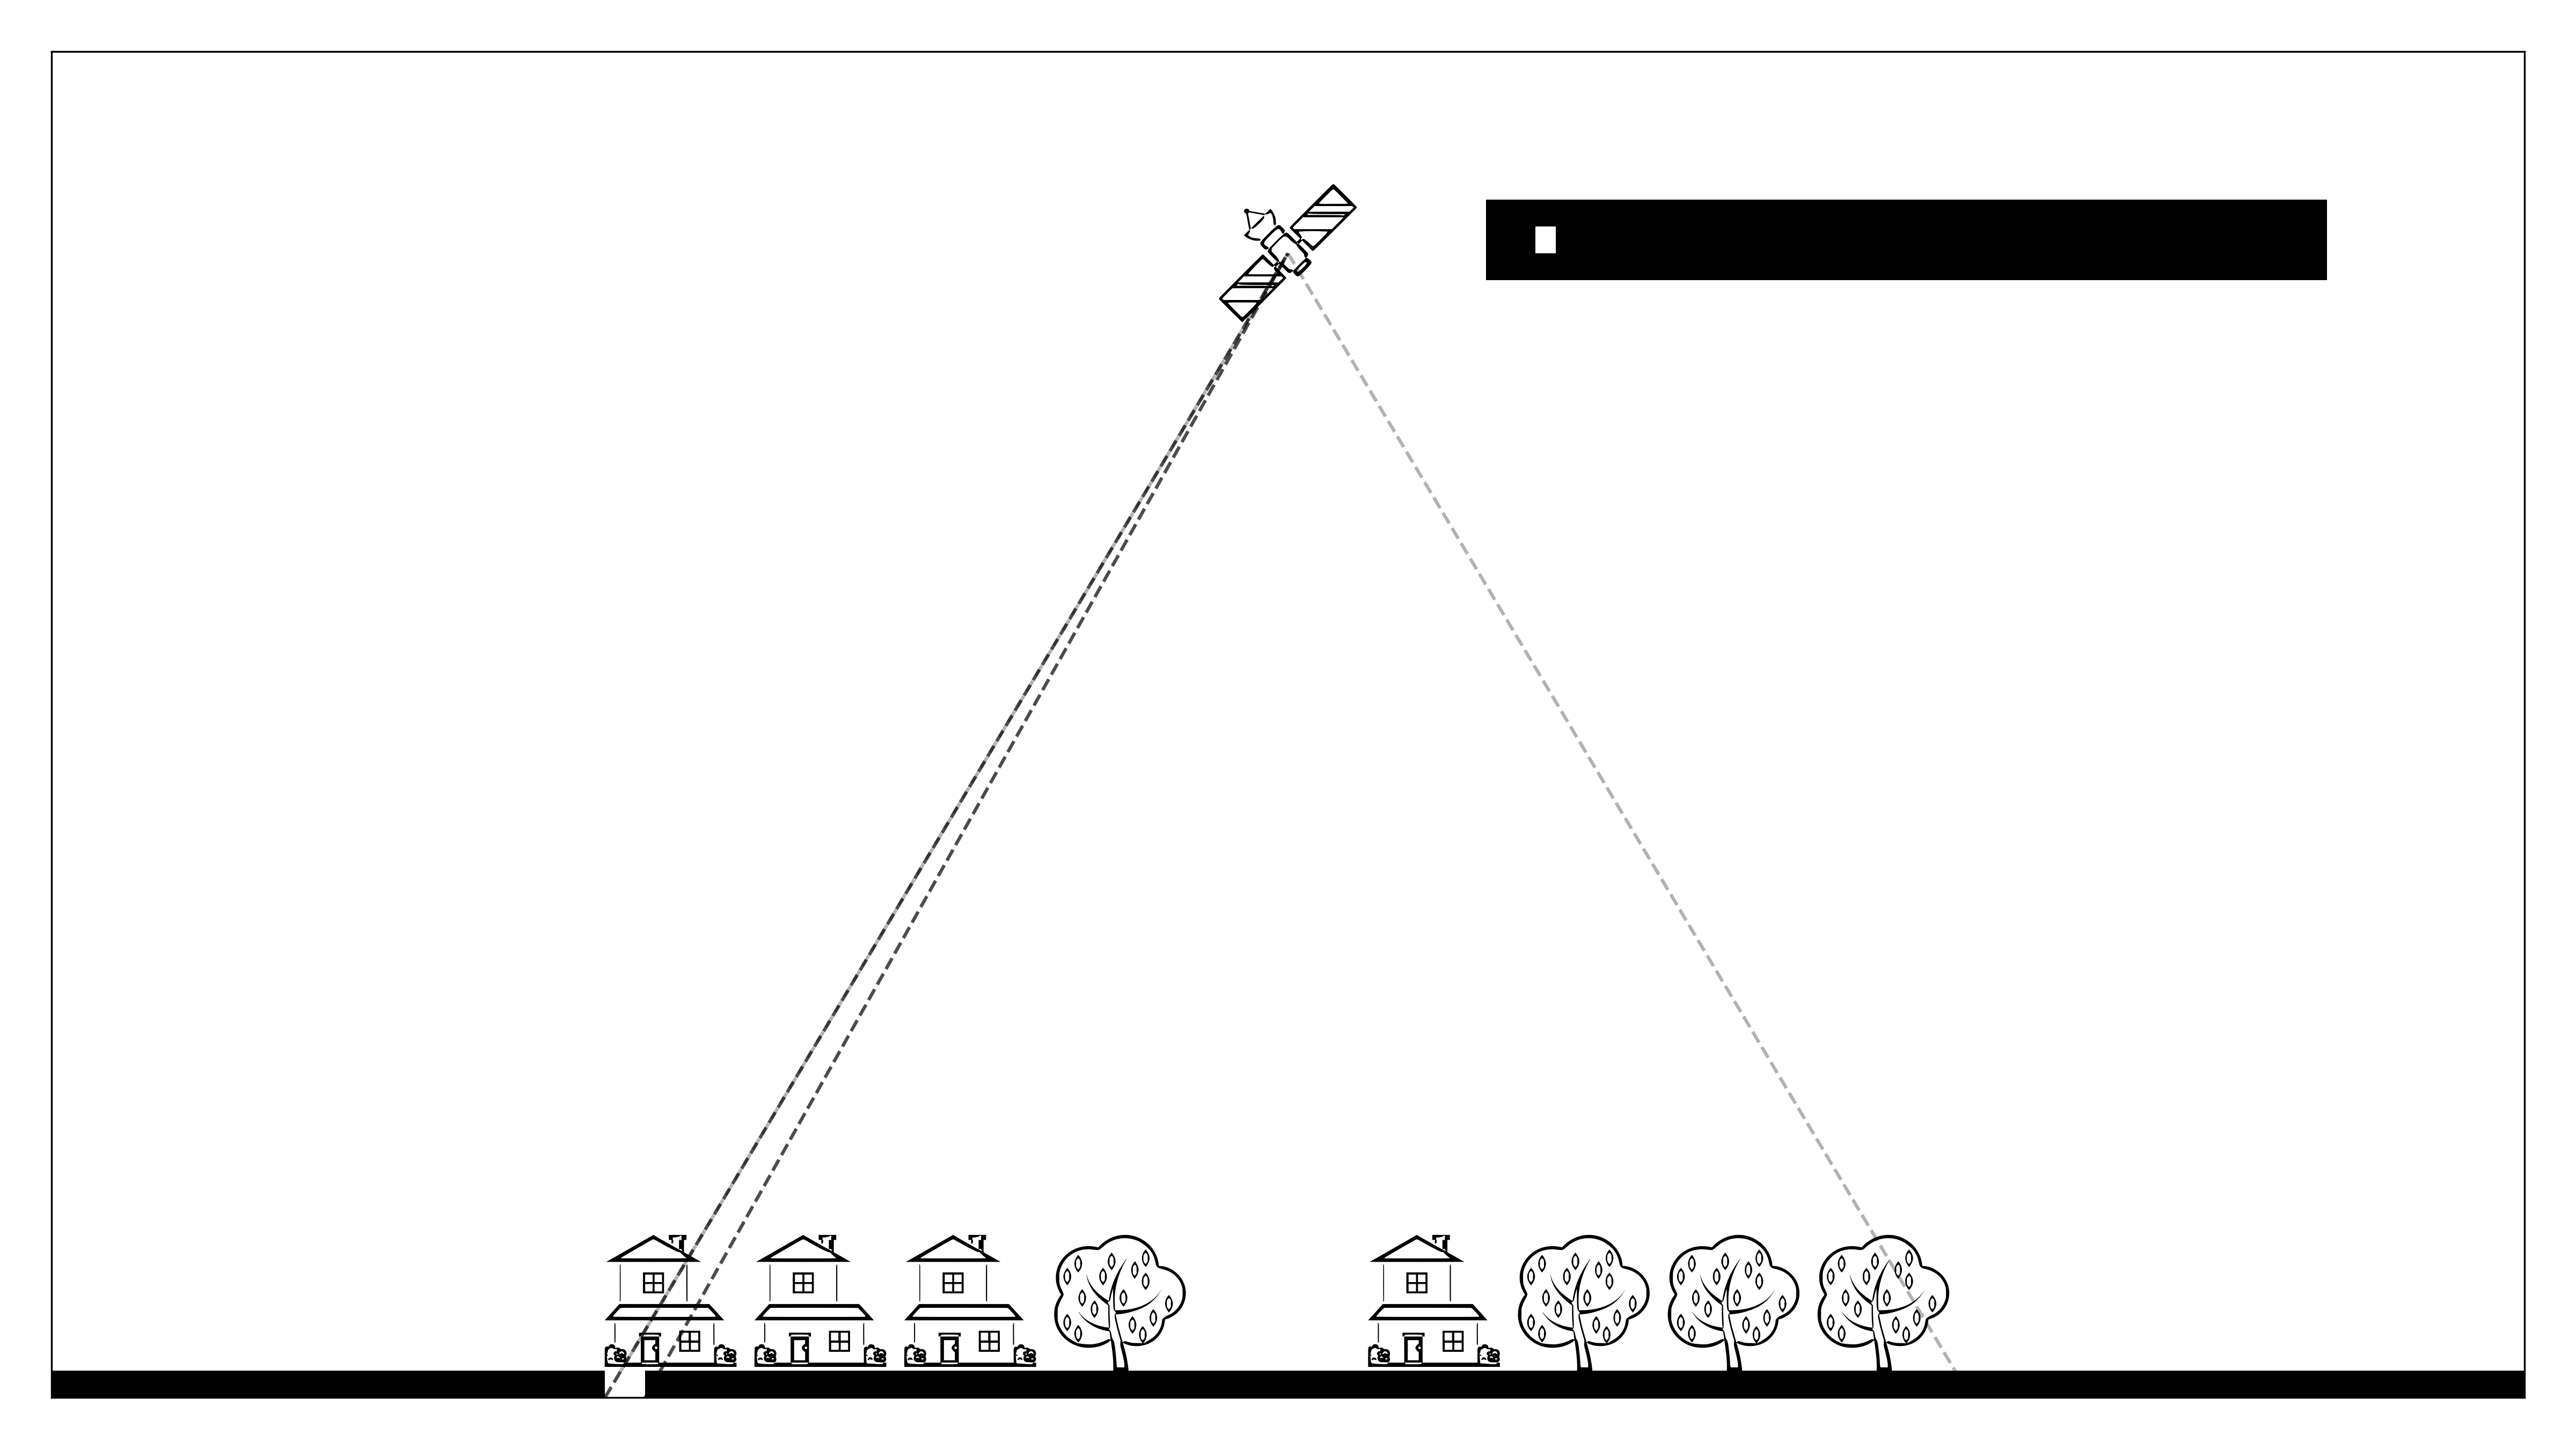
\includegraphics[width=0.8\textwidth]{fig:pixel1.png}}{./figs/fig:pixel1.mp4}
    \caption{Resolución proyectada en el terreno.}
    \label{}
  \end{figure}
\end{frame}


%--- Next Frame ---%

\begin{frame}{}
    \begin{figure}[h!]
        \centering
        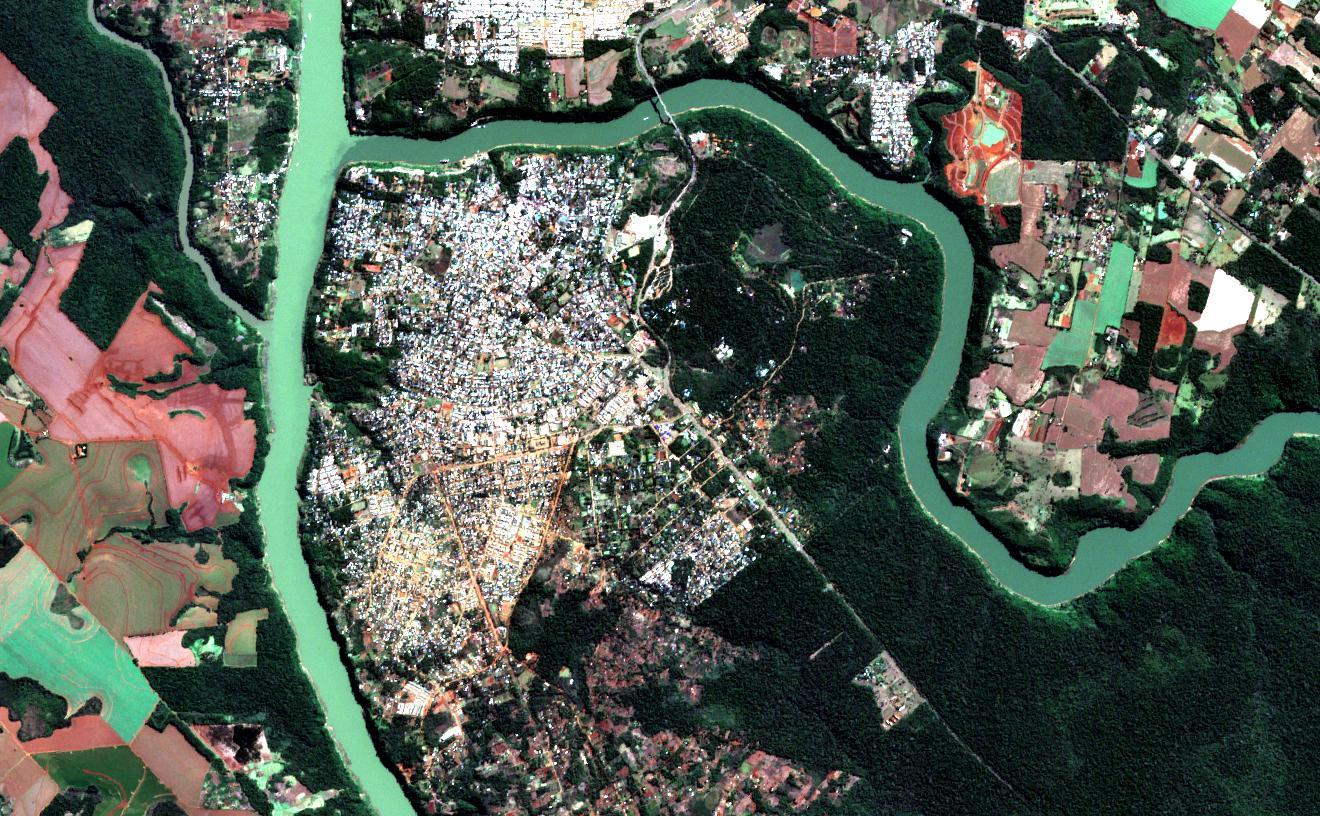
\includegraphics[width=0.7\textwidth]{fig:10m.jpg}
        \caption{Imagen con resolución espacial de 10m.}
    \end{figure}
\end{frame}
%--- Next Frame ---%

\begin{frame}{}
    \begin{figure}[h!]
        \centering
        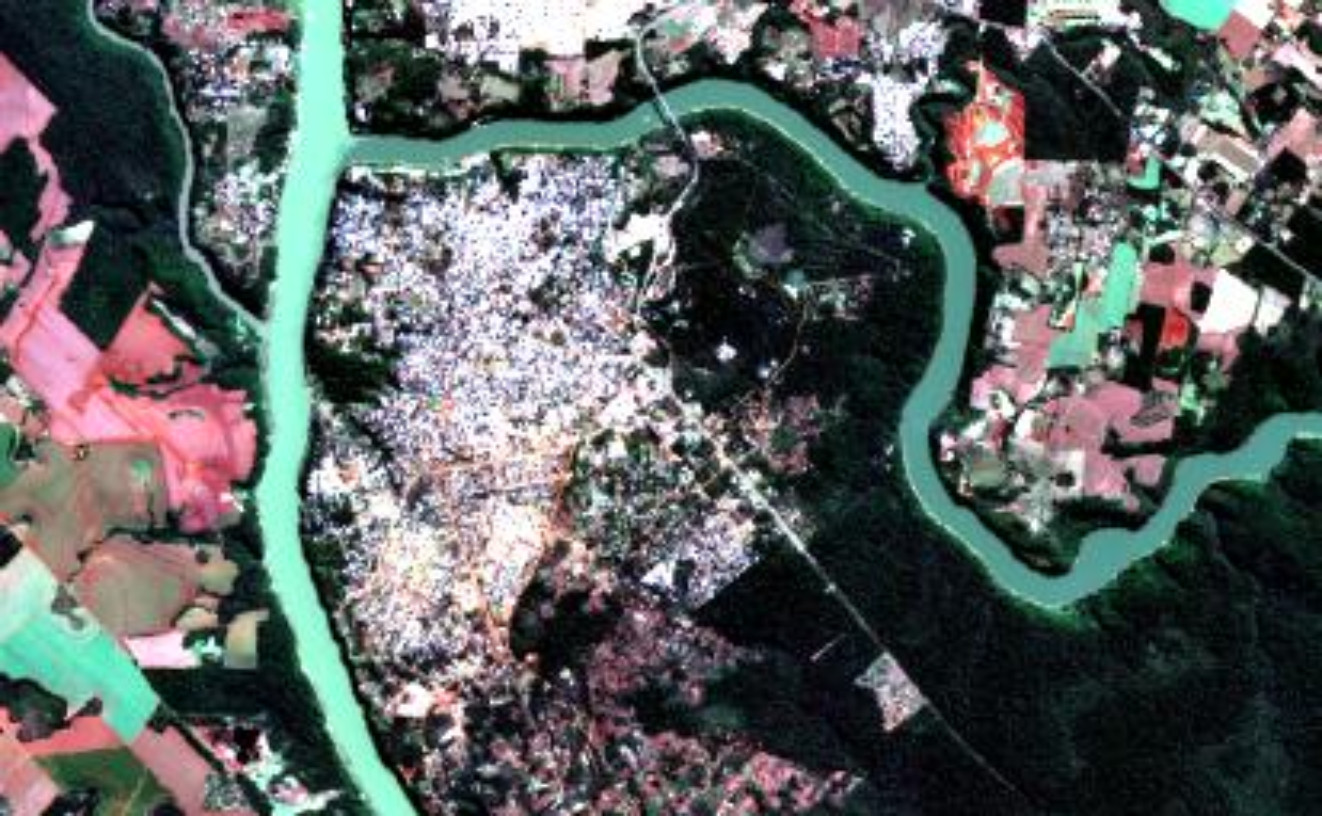
\includegraphics[width=0.7\textwidth]{fig:30m.jpg}
        \caption{Imagen con resolución espacial de 30m.}
    \end{figure}
\end{frame}
%--- Next Frame ---%

\begin{frame}{}
    \begin{figure}[h!]
        \centering
        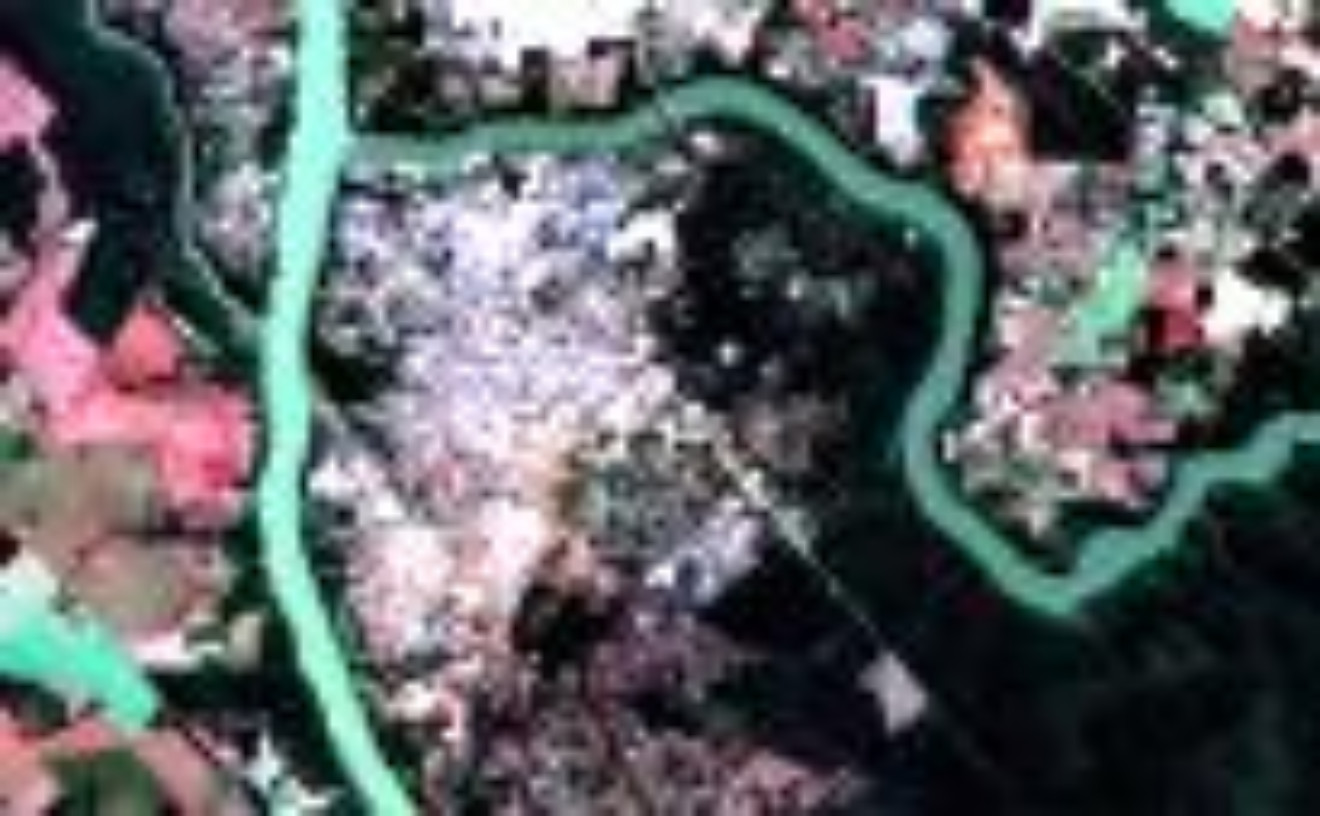
\includegraphics[width=0.7\textwidth]{fig:90m.jpg}
        \caption{Imagen con resolución espacial de 90m.}
    \end{figure}
\end{frame}
%--- Next Frame ---%

\begin{frame}{}
    \begin{figure}[h!]
        \centering
        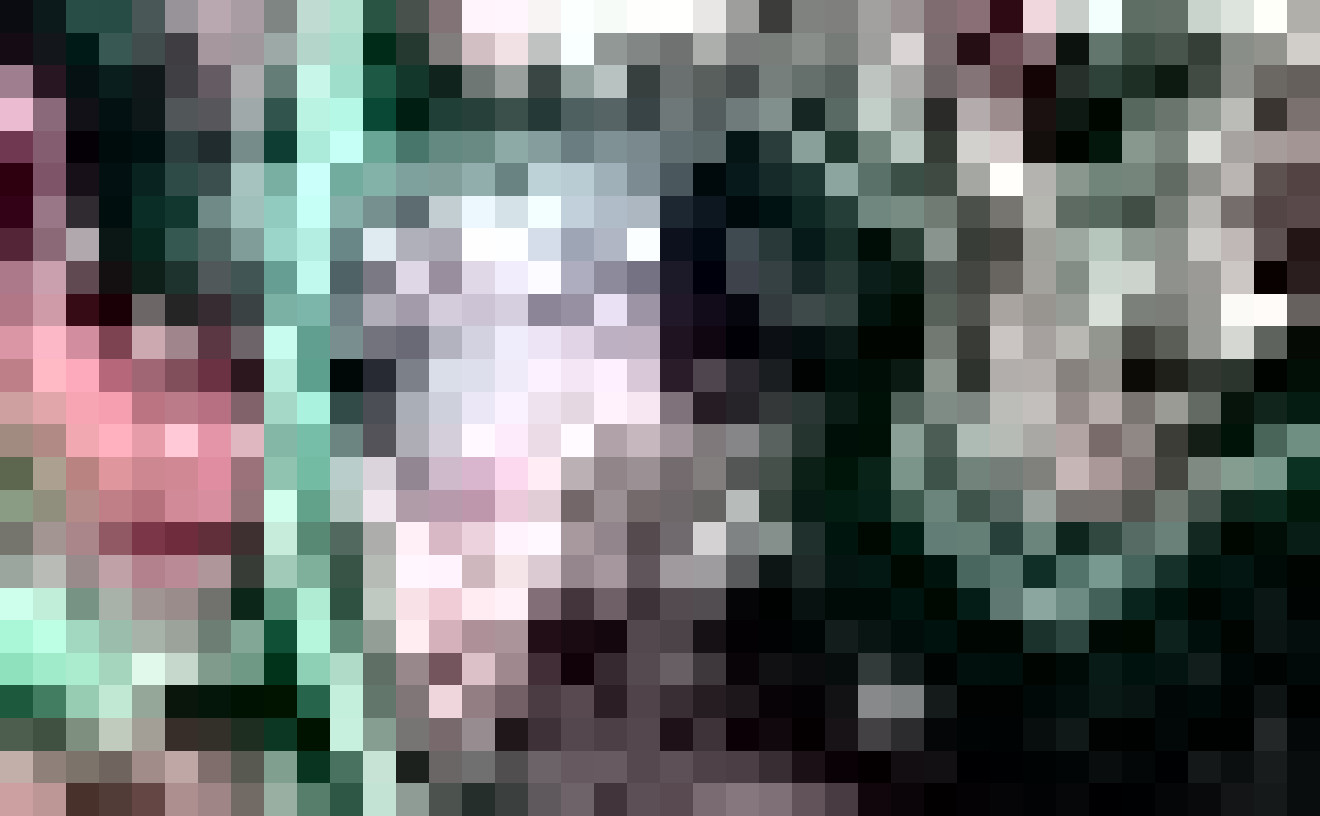
\includegraphics[width=0.7\textwidth]{fig:300m.jpg}
        \caption{Imagen con resolución espacial de 300m.}
    \end{figure}
\end{frame}
%--- Next Frame ---%

\begin{frame}{}
    \begin{figure}[h!]
        \centering
        
\includegraphics[width=0.7\textwidth]{fig:1000m.jpg}
        \caption{Imagen con resolución espacial de 1000m.}
    \end{figure}
\end{frame}
%--- Next Frame ---%
%--- Next Frame ---%
\begin{frame}{}
\only<1>{Resolución temporal.}

\end{frame}

\begin{frame}{}
    \begin{block}{Definición}
        Es el tiempo de revisita.
    \end{block}
\end{frame}
%--- Next Frame ---%


\begin{frame}{}
    \begin{figure}[h!]
    \centering
    \movie[width = 0.6 \textwidth,loop]{\centering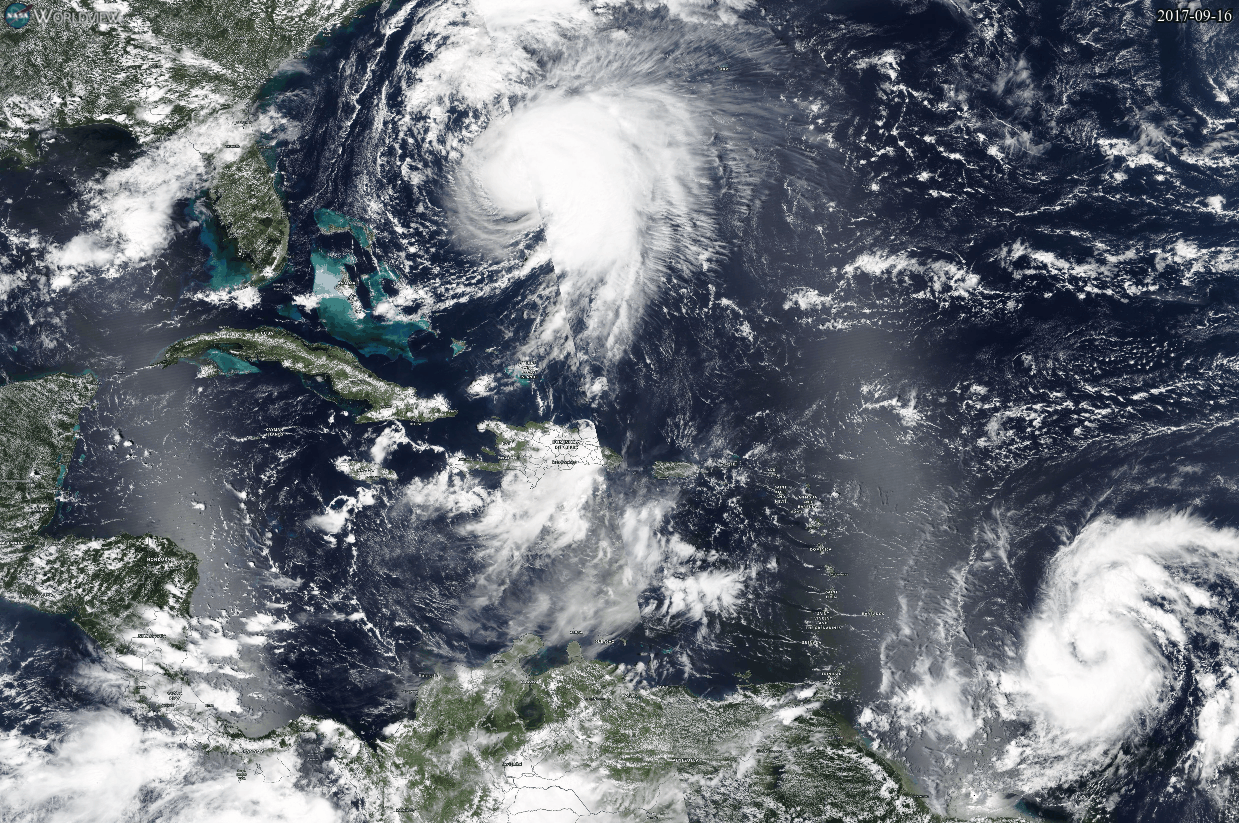
\includegraphics[width=0.6\textwidth]{fig:maria.png}}{./figs/fig:maria.mp4}
    \caption{Evolución del huracán María en el mes de septiembre de 2017. (\href{https://goo.gl/M5595z}{https://goo.gl/M5595z}).}
    \end{figure}
\end{frame}

%--- Next Frame ---%

\begin{frame}{}
    \begin{figure}[h!]
        \centering
        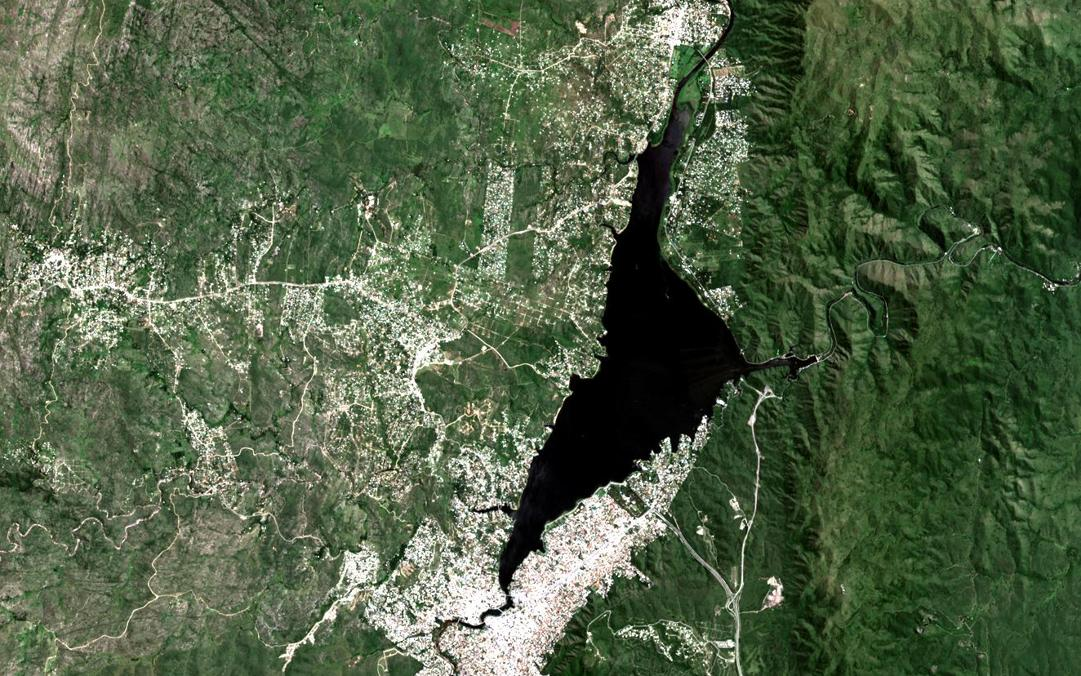
\includegraphics[width=0.6\textwidth]{fig:lake-beg.jpeg}
        \caption{Evolución temporal del contenido de clorofila en la superficie en el lago San Roque, en la provincia de Córdoba. Imagen del 12 de febrero de 2017.}
        \label{fig:lake-beg}
    \end{figure}
\end{frame}
%--- Next Frame ---%

\begin{frame}{}
    \begin{figure}[h!]
        \centering
        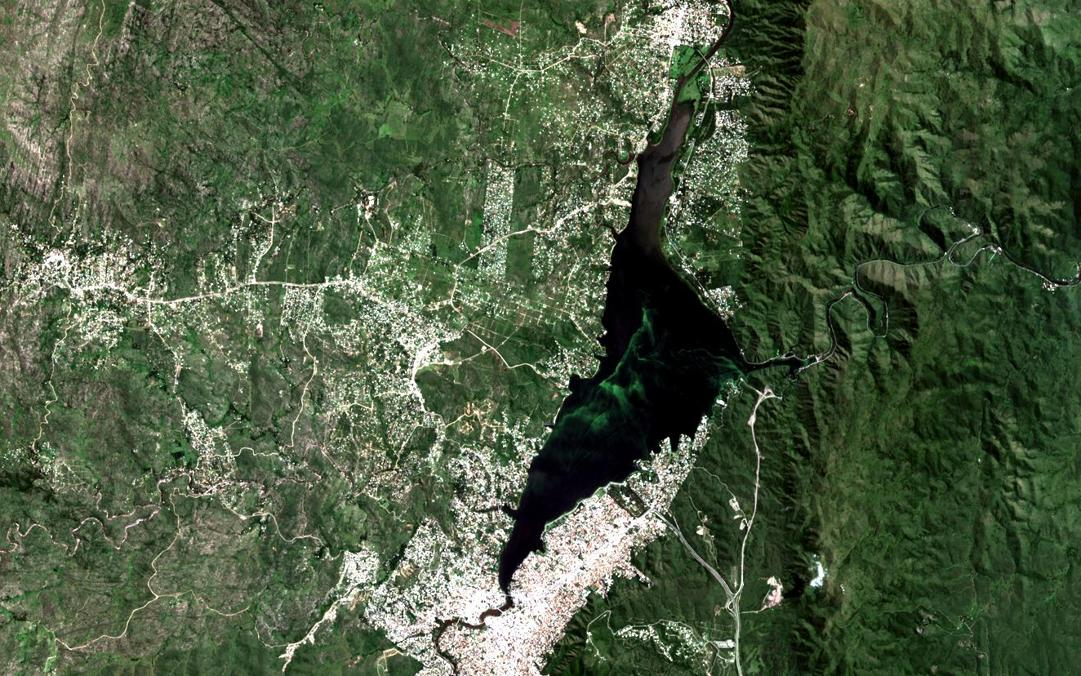
\includegraphics[width=0.6\textwidth]{fig:lake-end.jpeg}
        \caption{Evolución temporal del contenido de clorofila en la superficie en el lago San Roque. Imagen del 22 de febrero de 2017.}
        \label{fig:lake-end}
    \end{figure}
\end{frame}
%--- Next Frame ---%

\begin{frame}{}
    \begin{figure}[h!]
        \centering
        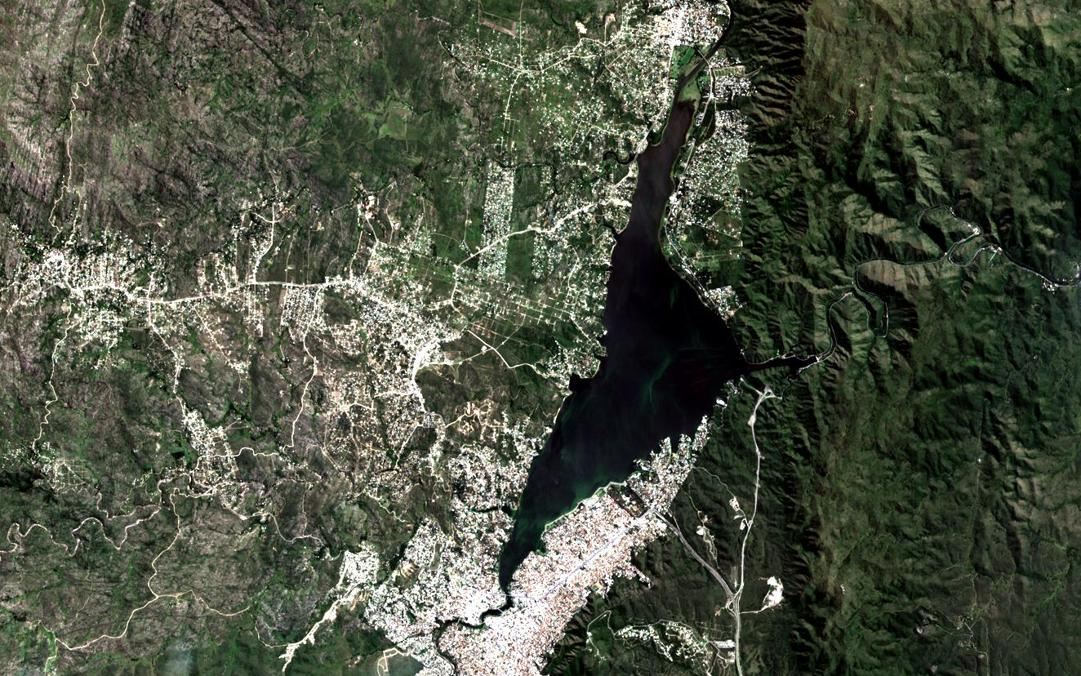
\includegraphics[width=0.6\textwidth]{fig:lake-aft.jpeg}
        \caption{Evolución temporal del contenido de clorofila en la superficie en el lago San Roque. Imagen del 14 de marzo de 2017. (\href{https://goo.gl/M5595z}{https://goo.gl/M5595z}).}
        \label{fig:lake-aft}
    \end{figure}
\end{frame}

%--- Next Frame ---%

\begin{frame}{}
    \begin{figure}[h!]
        \centering
        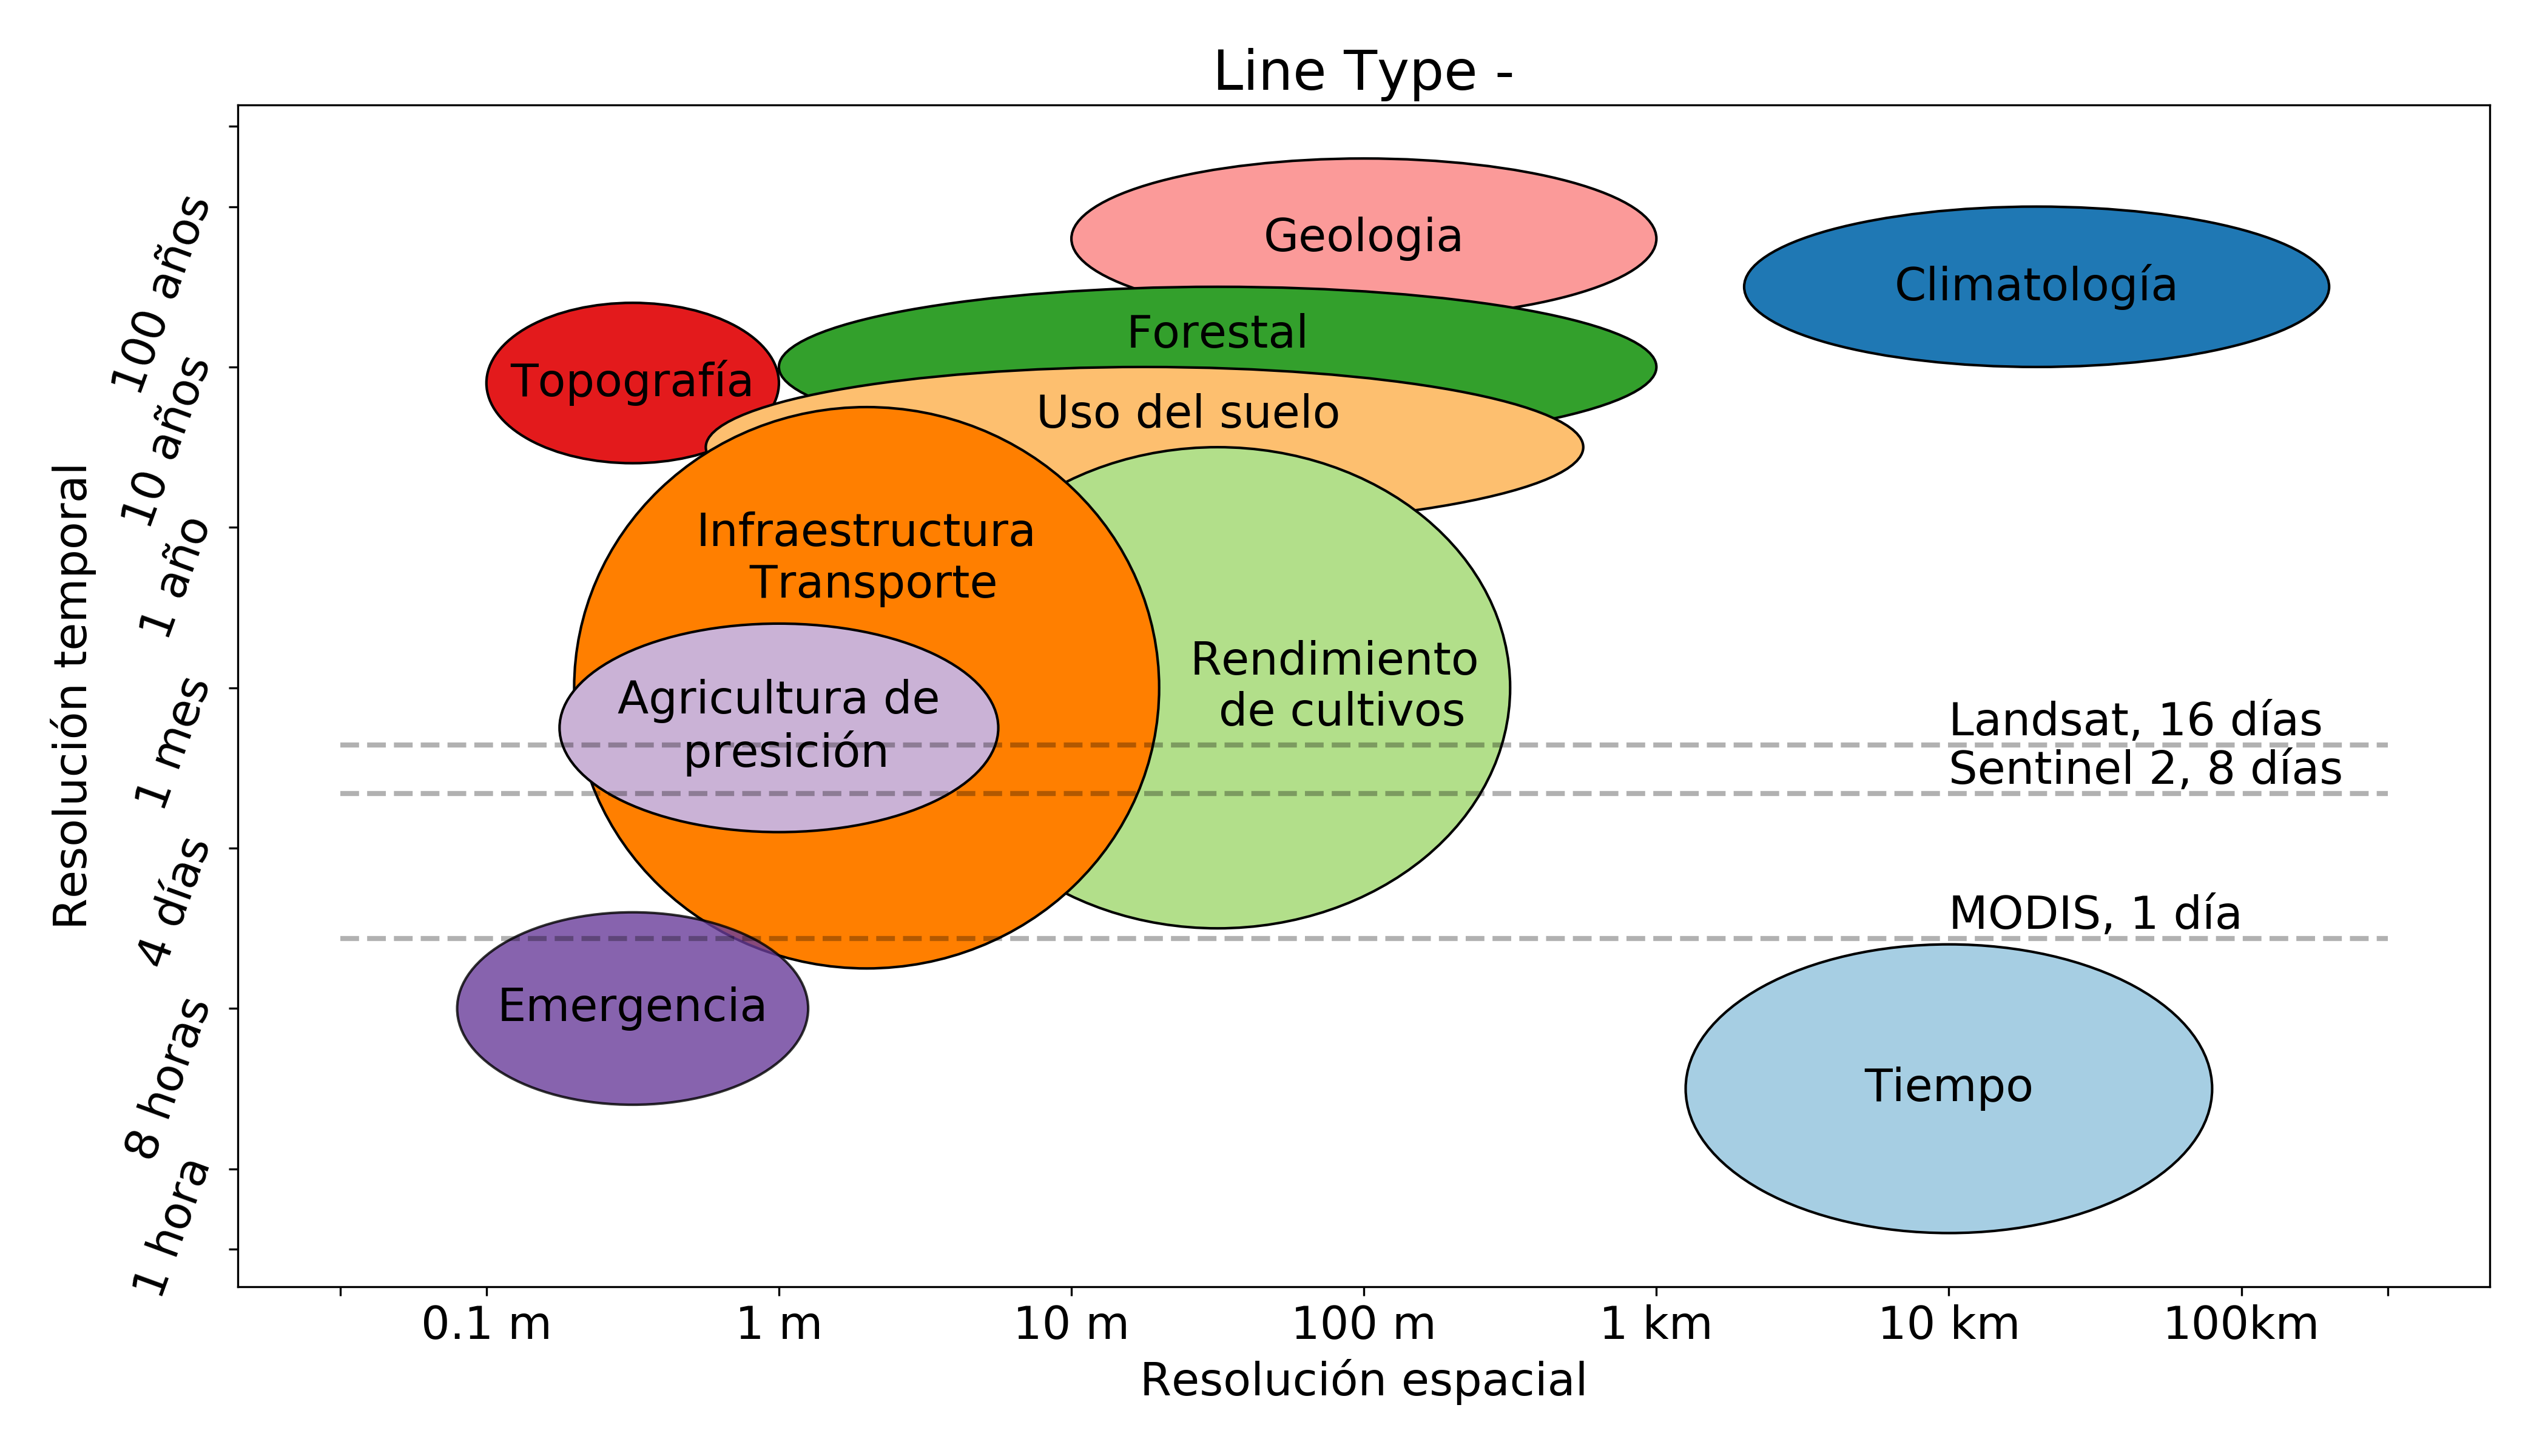
\includegraphics[width=0.7\textwidth]{fig:evst.png}
        \caption{Comparación de distintos usos de productos satelitales por resolución espacial y temporal.}
        \label{fig:evst}
    \end{figure}
\end{frame}
%--- Next Frame ---%

\gracias
%--- Next Frame ---%
